\documentclass[12pt]{article}

\usepackage{multirow}
\usepackage{amsmath}
\usepackage{amsfonts}
\usepackage{float}
\usepackage{fancyhdr}
\usepackage{graphicx}
\usepackage{setspace}
\usepackage{subcaption}
\usepackage{booktabs}
\usepackage{bm}
\usepackage[colorlinks=true,linkcolor=blue, citecolor=red]{hyperref}
\usepackage{url}
\usepackage[top=.75in, left=.75in, right=.75in, bottom=1in]{geometry}
\usepackage[utf8]{vietnam}

% For algorithm
\usepackage{mathtools}
\usepackage{algorithm}
 \usepackage[noend]{algpseudocode}
 \usepackage{setspace, etoolbox, caption}

\usepackage{algpseudocode}


% ============ CODE ============
\usepackage{listingsutf8}%\usepackage{listings}
\usepackage{xcolor}
\definecolor{codegreen}{rgb}{0,0.6,0}
\definecolor{codegray}{rgb}{0.5,0.5,0.5}
\definecolor{codepurple}{rgb}{0.58,0,0.82}
\definecolor{backcolour}{rgb}{0.95,0.95,0.92}

% Styling for the code.
\lstdefinestyle{mystyle}{
    backgroundcolor=\color{backcolour},   
    commentstyle=\color{codegreen},
    keywordstyle=\color{magenta},
    numberstyle=\tiny\color{codegray},
    stringstyle=\color{codepurple},
    basicstyle=\ttfamily\footnotesize,
    breakatwhitespace=false,         
    breaklines=true,                 
    captionpos=b,                    
    keepspaces=true,                 
    numbers=left,                    
    numbersep=5pt,                  
    showspaces=false,                
    showstringspaces=false,
    showtabs=false,                  
    tabsize=2
}
\lstset{style=mystyle}

% Disable indentation on new paragraphs
%\setlength{\parindent}{0pt}

% Line spacing 1.5
\renewcommand{\baselinestretch}{1}

% Optional: graphic path
% \graphicspath{PATH_TO_GRAPHIC_FOLDER}

% To use Times font family, uncomment this row
% \usepackage{mathptmx}

% To use roman section / subsection, uncomment these rows
% \renewcommand{\thesection}{\Roman{section}}
% \renewcommand{\thesubsection}{\thesection.\Roman{subsection}}

% Define course name, report name and report title.
\newcommand{\coursename}{Phương pháp Toán cho Trí tuệ nhân tạo}
\newcommand{\reportname}{CLIP (Contrastive Language-Image Pretraining)}
\newcommand{\reporttitle}{Final Project}
\newcommand{\studentname}{Nguyễn Đình Hà Dương (23122002)\\Nguyễn Lê Hoàng Trung (23122004)\\Đinh Đức Tài (23122013)\\Hoàng Minh Trung (23122014)}
\newcommand{\teachername}{TS. Cấn Trần Thành Trung\\ThS. Nguyễn Ngọc Toàn}

\newcommand{\leftfooter}{\LaTeX\ by \href{https://github.com/ductai05}{Duc Tai Dinh}}

% ============ HEADER AND FOOTER ============
% Header length
\setlength{\headheight}{29.43912pt}

% Footer page number would be on the lower-right corner
\pagestyle{fancy}
\fancyfoot{}
\fancyfoot[R]{Trang \thepage}

\lhead{Final project: CLIP}
\rhead{
Trường Đại học Khoa học Tự nhiên - ĐHQG HCM\\
\coursename
}
\lfoot{\leftfooter}

% ============ DOCUMENT ============
\begin{document}
\begin{titlepage}
\newcommand{\HRule}{\rule{\linewidth}{0.5mm}}
\centering

\textsc{\LARGE đại học quốc gia tphcm}\\[1.5cm]
\textsc{\Large trường đại học khoa học tự nhiên}\\[0.5cm]
\textsc{\large khoa công nghệ thông tin}\\[0.5cm]
\textsc{AI23 (23TNT1), FIT@HCMUS-VNUHCM}\\[0.5cm]

\HRule \\[0.4cm]
{ 
\huge{\bfseries{\reporttitle}}\\[0.5cm]
\large{\bfseries{Đề tài: \reportname}}
}\\[0.4cm]
\HRule \\[0.5cm]

\textbf{\large Môn học: \coursename}\\[0.5cm]

\begin{minipage}[t]{0.5\textwidth}
\begin{flushleft} \large
\emph{Sinh viên thực hiện:}\\
\studentname
\end{flushleft}
\end{minipage}
~
\begin{minipage}[t]{0.4\textwidth}
\begin{flushright} \large
\emph{Giáo viên hướng dẫn:} \\
\teachername
\end{flushright}
\end{minipage}\\[1.5cm]

{\large \today}\\[0.5cm]


\includegraphics[scale=.3]{img/hcmus-logo.png}\\[1cm] 

\vfill
\end{titlepage}
	
	
\tableofcontents
\pagebreak

\newpage
\section{Giới thiệu}

\paragraph{}{Đây là bài báo cáo cho \textbf{Lab 1 - Dự đoán giá xe}, môn Phương pháp toán cho Trí tuệ nhân tạo, lớp Trí tuệ nhân tạo Khóa 2023 (23TNT1), Khoa Công nghệ thông tin, Trường Đại học Khoa học tự nhiên - Đại học Quốc gia TP.HCM. Trong bài báo cáo này, chúng tôi sẽ trình bày phương pháp \textbf{dự đoán giá xe} bằng \textbf{mô hình hồi quy tuyến tính} dựa trên dữ liệu huấn luyện được cho trước.}

\paragraph{}{\textbf{Báo cáo được thực hiện bởi nhóm các thành viên:}} 
\begin{itemize}
    \item Nguyễn Đình Hà Dương (23122002)
    \item Nguyễn Lê Hoàng Trung (23122004)
    \item Đinh Đức Tài (23122013)
    \item Hoàng Minh Trung (23122014)
\end{itemize}

\paragraph{}{\textbf{Đường dẫn repository Github của báo cáo:}} \href{https://github.com/ductai05/Math-For-AI}{https://github.com/ductai05/Math-For-AI} \cite{repo}

\paragraph{}{\textbf{Bảng phân công nhiệm vụ cho từng thành viên:}}

\begin{table}[H]
\centering
\renewcommand{\arraystretch}{1.4}
\label{tab:phancongnv}
\begin{tabular}{|c|c|l|}
\hline
\textbf{Họ và tên} & \textbf{MSSV} & \multicolumn{1}{c|}{\textbf{Nhiệm vụ}} \\ \hline
\begin{tabular}[c]{@{}c@{}}Nguyễn Đình \\ Hà Dương\end{tabular} &
  23122002 &
  \begin{tabular}[c]{@{}l@{}}- Linear regression với phương pháp PCA.\\ - Cơ sở toán học của Linear regression \& Ridge regression \& PCA.\end{tabular} \\ \hline
\begin{tabular}[c]{@{}c@{}}Nguyễn Lê \\ Hoàng Trung\end{tabular} &
  23122004 &
  \begin{tabular}[c]{@{}l@{}}- Polynomial linear regression.\\ - Cơ sở toán học của Polynomial linear regression. Code testing.\end{tabular} \\ \hline
\begin{tabular}[c]{@{}c@{}}Đinh \\ Đức Tài\end{tabular} &
  23122013 &
  \begin{tabular}[c]{@{}l@{}}- Data preprocessing, visualization, encoding, normalization.\\ - Simple linear regression \& Evaluation metrics. Review report.\end{tabular} \\ \hline
\begin{tabular}[c]{@{}c@{}}Hoàng \\ Minh Trung\end{tabular} &
  23122014 &
  \begin{tabular}[c]{@{}l@{}}- Multiple linear regression \\ - Cơ sở toán học của Multiple linear regression \& Lasso regression\end{tabular} \\ \hline
\end{tabular}
\end{table}

\paragraph{}{\textbf{Các thư viện và công nghệ sử dụng:}}

\begin{itemize}
    \item Numpy: thư viện Python để xử lý số học.
    \item Pandas: thư viện Python để thao tác và xử lý dữ liệu.
    \item Matplotlib: thư viện Python để trực quan hóa dữ liệu.
    \item Jupyter Notebook (thông qua jupyter, ipykernel): Môi trường làm việc tương tác cho phép kết hợp mã thực thi, văn bản mô tả (Markdown), công thức toán học và trực quan hóa trong cùng một tài liệu.
    \item Visual Studio Code: Trình soạn thảo mã nguồn (IDE). 
    \item Git, Github: Quản lý dự án, lưu và chia sẻ source code.
\end{itemize}

\pagebreak
\section{Lý do lựa chọn}

\paragraph{}{Trong hai hướng dự án được cho trước, chúng tôi lựa chọn \textbf{Hướng 2: Nghiên cứu một bài báo khoa học} với lý do sau:}

\begin{itemize}
    \item Nâng cao hiểu biết về các mô hình cơ bản, quan trọng trong lĩnh vực Machine learning / Deep learning / AI. 
    \item Hiểu cách ứng dụng của toán học và kĩ thuật lập trình trong nghiên cứu và thực tế.
    \item Tăng khả năng tự nghiên cứu và áp dụng tri thức mới vào thực tiễn.
    \item Nâng cao tư duy phản biện, phân tích, tổng hợp.
\end{itemize}

\paragraph{}{\textbf{CLIP} \cite{radford2021learning} (Contrastive Language-Image Pre-Training) là một mạng nơ-ron được huấn luyện trên nhiều cặp dữ liệu (ảnh, văn bản). Mô hình này có thể được hướng dẫn bằng ngôn ngữ tự nhiên để dự đoán đoạn văn bản phù hợp nhất với một hình ảnh, mà không cần được tối ưu hóa trực tiếp cho nhiệm vụ đó — tương tự như khả năng “zero-shot” (không cần huấn luyện lại) của GPT-2 và GPT-3.\\

CLIP đạt hiệu suất tương đương với ResNet-50 gốc trên bộ dữ liệu ImageNet theo cách “zero-shot”, mà không cần sử dụng bất kỳ ví dụ có gán nhãn nào trong 1,28 triệu ảnh ban đầu, từ đó vượt qua một số thách thức lớn trong lĩnh vực thị giác máy tính.\\

Paper \cite{radford2021learning}, code \cite{code_clip} và blog \cite{blog_clip} của CLIP được trích dẫn dưới phần tài liệu.
}

\paragraph{}{\textbf{Lý do lựa chọn bài báo:}}

\begin{itemize}
    \item CLIP là một mô hình cơ sở (foundation model) quan trọng trong lĩnh vực học đa phương thức, kết nối giữa thị giác máy tính và xử lý ngôn ngữ tự nhiên.
    \item CLIP có ứng dụng đa dạng: truy vấn hình ảnh bằng văn bản; phân loại hình ảnh zero-shot và fewshot; phân tích nội dung video.
    \item CLIP được xây dựng dựa trên các kiến thức nền tảng toán học như đại số tuyến tính, xác suất thống kê. Hiểu rõ CLIP sẽ nâng cao kiến thức về toán học.
\end{itemize}

\paragraph{}{\textbf{Kế hoạch thực hiện:}

\begin{enumerate}
    \item Phân tích các nền tảng của CLIP: WIT, Contrastive learning, Vision Transformer/Transformer, Embedding Vector Space,...
    \item Phân tích dữ liệu, cách huấn luyện CLIP, so sánh các mô hình.
    \item Ứng dụng của CLIP: truy vấn ảnh dựa trên văn bản đầu vào (text-to-image).
    \item Phân tích các mô hình VLMs tương tự CLIP: ALIGN, BLIP, ... 
    
\end{enumerate}
\newpage
\section{Nền tảng xây dựng mô hình CLIP}

\subsection{Bộ dữ liệu WIT (WebImageText)}
\subsubsection{Bối cảnh và thách thức của các bộ dữ liệu truyền thống}
\paragraph{}{Trong nhiều năm, các mô hình thị giác máy tính hàng đầu đã được huấn luyện trên các bộ dữ liệu được gán nhãn thủ công như ImageNet (phân loại đối tượng), MS-COCO (phát hiện đối tượng và chú thích), hay OpenImages. Mặc dù những bộ dữ liệu này đã thúc đẩy sự tiến bộ vượt bậc, chúng tồn tại những hạn chế đáng kể:}
\begin{itemize}
\item \textbf{Quy mô và chi phí hạn chế:} Việc gán nhãn thủ công hàng triệu hình ảnh là một quá trình tốn kém và mất thời gian. Điều này giới hạn quy mô của bộ dữ liệu, khiến chúng không thể bao phủ toàn bộ sự đa dạng của thế giới thị giác.
\item \textbf{Phạm vi khái niệm cố định:} Các bộ dữ liệu này thường tập trung vào một tập hợp các danh mục cố định (ví dụ: 1000 lớp trên ImageNet-1K). Điều này khiến mô hình học được một bộ kỹ năng rất cụ thể và gặp khó khăn khi tổng quát hóa sang các khái niệm hoặc đối tượng chưa từng thấy trong quá trình huấn luyện. Chúng thiếu khả năng \textbf{open set recognition} (nhận diện khái niệm tổng quát).
\item \textbf{Thiếu ngữ cảnh và sắc thái:} Một nhãn đơn lẻ như "mèo" không truyền tải được nhiều thông tin như một chú thích mô tả chi tiết: "một con mèo Xiêm đang nằm trên ghế sofa dưới trời nắng". Sự thiếu hụt ngữ cảnh này giới hạn độ sâu của biểu diễn mà mô hình có thể học được.
\end{itemize}
\paragraph{}{Trong khi đó, lĩnh vực xử lý ngôn ngữ tự nhiên đã chứng kiến một cuộc cách mạng nhờ các mô hình được huấn luyện trên khối lượng văn bản khổng lồ từ internet (ví dụ: GPT-3, BERT). Câu hỏi đặt ra là: liệu chúng ta có thể áp dụng triết lý tương tự - sử dụng dữ liệu "thô" từ web với sự giám sát bằng ngôn ngữ tự nhiên - để đạt được bước đột phá tương tự trong thị giác máy tính? Bộ dữ liệu WIT ra đời để trả lời câu hỏi này.}
\subsubsection{Giải pháp Natural Language Supervision}
\paragraph{}{WIT được xây dựng để trở thành nền tảng cho việc học biểu diễn hình ảnh từ ngôn ngữ tự nhiên. Nó khác biệt rõ rệt so với các bộ dữ liệu truyền thống ở ba khía cạnh chính: quy mô, bản chất giám sát và chiến lược xây dựng.}
\paragraph{Quy mô vượt trội}
WIT bao gồm \textbf{400 triệu cặp (hình ảnh, văn bản)} được thu thập từ internet. Con số này lớn hơn gấp nhiều lần so với các bộ dữ liệu học sâu thị giác tiêu chuẩn:
\begin{itemize}
\item So với ImageNet (khoảng 1.28 triệu hình ảnh huấn luyện), WIT lớn hơn khoảng 300 lần về số lượng cặp.
\item So với MS-COCO (khoảng 118.000 hình ảnh huấn luyện), WIT lớn hơn khoảng 4000 lần.
\end{itemize}
\paragraph{}{Sự "khổng lồ" về quy mô này là một yếu tố mang tính quyết định. Nó cho phép mô hình:}
\begin{itemize}
\item \textbf{Tiếp xúc đa dạng hơn:} Gặp gỡ hàng tỷ đối tượng, ngữ cảnh, phong cách hình ảnh, và mô tả văn bản khác nhau. Điều này giúp mô hình không chỉ học các đặc trưng cấp thấp mà còn cả các tính chất, khái niệm trừu tượng, phức tạp.
\item \textbf{Giảm thiểu overfitting:} Với một lượng dữ liệu đồ sộ, khả năng mô hình "ghi nhớ" các ví dụ cụ thể hoặc các mối tương quan giả mạo trong dữ liệu huấn luyện giảm đi đáng kể, buộc nó phải học các khái niệm tổng quát hơn.
\item \textbf{Học hỏi sâu sắc hơn:} Khối lượng dữ liệu lớn cho phép huấn luyện các mô hình có năng lực lớn (ví dụ: hàng tỷ tham số) một cách hiệu quả, khai thác tối đa tiềm năng của kiến trúc mạng sâu.
\end{itemize}
\paragraph{Natural Language Supervision}
Đây là điểm đặc biệt và cốt lõi nhất của WIT. Thay vì sử dụng các nhãn phân loại đơn lẻ (như "chó", "mèo"), WIT sử dụng \textbf{văn bản mô tả tự nhiên} đi kèm với hình ảnh (ví dụ: chú thích, mô tả, văn bản từ các trang web).
\begin{itemize}
\item \textbf{Tính đa dạng và khả năng khái quát hóa của khái niệm:}
\begin{itemize}
\item Ngôn ngữ tự nhiên có khả năng mô tả \textbf{vô số khái niệm} - từ đối tượng, hành động, thuộc tính, đến ngữ cảnh và mối quan hệ - mà không bị giới hạn bởi một danh sách cố định. Một hình ảnh có thể được mô tả cụ thể bằng "một con chó Husky đang bơi trong hồ", thay vì chỉ là "chó".
\item Khả năng này là chìa khóa cho \textit{Zero-Shot Transfer} của CLIP. Khi mô hình học cách liên kết hình ảnh với các mô tả ngôn ngữ đa dạng, nó có thể nhận diện các khái niệm mới (chưa từng thấy trong quá trình huấn luyện) chỉ bằng cách mô tả chúng bằng văn bản.
\end{itemize}
\item \textbf{Tiết kiệm chi phí:}
\begin{itemize}
\item Dữ liệu WIT được thu thập tự động từ internet, loại bỏ nhu cầu về quá trình gán nhãn thủ công tốn kém. Điều này giúp giảm chi phí đáng kể và cho phép quy mô bộ dữ liệu tăng lên theo khả năng thu thập dữ liệu web.
\item Quá trình này mô phỏng cách con người học: chúng ta học về thế giới xung quanh thông qua các giác quan và sự mô tả bằng ngôn ngữ, chứ không phải chỉ qua các nhãn cố định.
\end{itemize}
\item \textbf{Chấp nhận "nhiễu" tự nhiên:}
\begin{itemize}
\item Dữ liệu từ internet thường chứa "nhiễu" và không được chọn lọc một cách hoàn hảo. Các cặp hình ảnh-văn bản có thể không luôn khớp chính xác (ví dụ: chú thích không liên quan trực tiếp đến nội dung chính của ảnh).
\item Tuy nhiên, các nhà nghiên cứu nhận thấy rằng việc học từ dữ liệu nhiễu này thực sự có lợi. Nó buộc mô hình phải học các biểu diễn mạnh mẽ hơn, ít bị ảnh hưởng bởi các mối tương quan giả mạo, và tổng quát hóa tốt hơn ra các phân phối dữ liệu thực tế (thường cũng không hoàn hảo). Điều này giúp CLIP có tính mạnh mẽ cao hơn đối với các dịch chuyển phân phối tự nhiên.
\end{itemize}
\end{itemize}
\paragraph{Chiến lược xây dựng bộ dữ liệu}
Mặc dù dữ liệu WIT được thu thập từ internet một cách tự động, quá trình này không hoàn toàn ngẫu nhiên mà được thực hiện một cách có chiến lược để đảm bảo tính bao quát. Các cặp hình ảnh-văn bản được tìm kiếm dựa trên một danh sách \textbf{500.000 truy vấn}. Danh sách này được xây dựng từ:
\begin{itemize}
\item Tất cả các từ xuất hiện ít nhất 100 lần trong phiên bản tiếng Anh của Wikipedia.
\item Các bigram (cặp từ) có thông tin tương hỗ điểm cao (high pointwise mutual information).
\item Tên của tất cả các bài viết Wikipedia trên một ngưỡng khối lượng tìm kiếm nhất định.
\item Tất cả các tập hợp từ WordNet (WordNet synsets) chưa có trong danh sách truy vấn.
\end{itemize}
\paragraph{}{Chiến lược này đảm bảo rằng bộ dữ liệu WIT bao phủ một \textbf{phạm vi rất rộng} các khái niệm, đối tượng, và tình huống mà mọi người quan tâm và mô tả trên web, từ đó cung cấp một nền tảng kiến thức thị giác-ngôn ngữ phong phú cho mô hình.}


\subsection{Kiến trúc mô hình}
\paragraph{}{Kiến trúc mô hình giúp CLIP học cách liên kết hình ảnh và văn bản trong một không gian nhúng chung. Thay vì phát triển một kiến trúc mới, họ đã \textbf{tận dụng và điều chỉnh các kiến trúc mạng có sẵn đạt hiệu quả cao}.
Về cơ bản, kiến trúc CLIP bao gồm hai bộ mã hóa (encoders) chính hoạt động độc lập để xử lý hai loại dữ liệu khác nhau:}
\begin{itemize}
\item \textbf{Bộ mã hóa hình ảnh (Image Encoder):} Chuyển đổi một hình ảnh thành một vector biểu diễn (embedding) trong không gian đa phương thức chung.
\item \textbf{Bộ mã hóa văn bản (Text Encoder):} Chuyển đổi một đoạn văn bản (chú thích) thành một vector biểu diễn (embedding) trong cùng không gian đa phương thức đó.
\end{itemize}
\paragraph{}{Sau đó, các embedding vector từ cả hai bộ mã hóa này sẽ được so sánh thông qua một phép nhân vô hướng để đo lường độ tương đồng, làm cơ sở cho \hyperref[subsec:contrastive_learning]{Contrastive learning} của CLIP.}
\subsubsection{Image Encoder}
\paragraph{}{Bộ mã hóa hình ảnh chịu trách nhiệm trích xuất các đặc trưng từ dữ liệu đầu vào. CLIP đã thử nghiệm hai dòng kiến trúc chính: \textbf{ResNet} và \textbf{Vision Transformer}.}
\paragraph{Dòng kiến trúc ResNet (Residual Networks)}
ResNet \hyperref[resnet]{(He et al., 2016a)} là một kiến trúc CNN mang tính đột phá, nổi tiếng với việc sử dụng kĩ thuật \textit{skip connections} giúp huấn luyện các mạng rất sâu: 
\begin{figure}[H]
\centering
    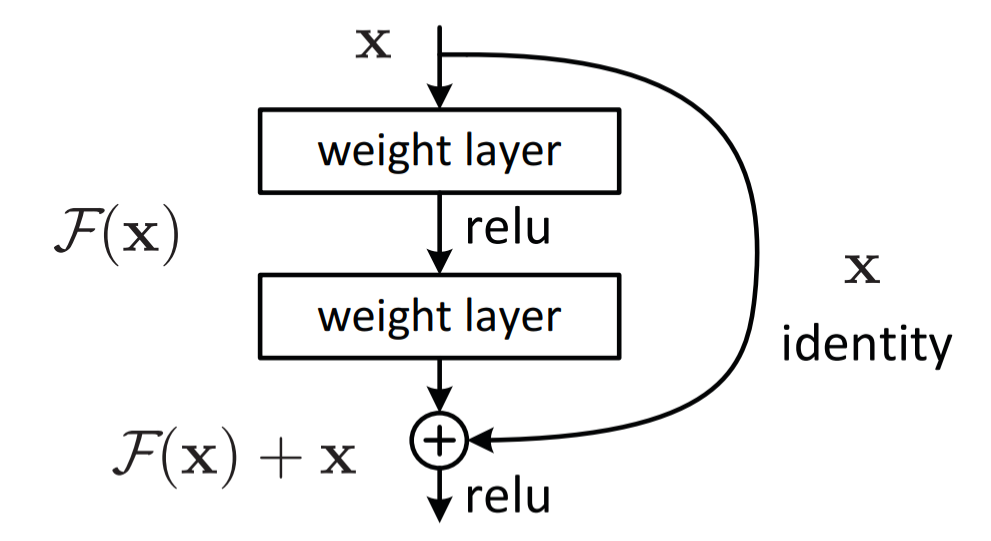
\includegraphics[width=0.7\textwidth]{img/03-skip_connection.png}
    \caption{Kiến trúc một residual block trong ResNet. Đầu vào $x$ được truyền trực tiếp qua một đường tắt (identity shortcut) và cộng với đầu ra $\mathcal{F} (x)$ của các lớp học trọng số. Skip connection giúp duy trì thông tin gốc, hỗ trợ truyền gradient hiệu quả và là yếu tố then chốt giúp huấn luyện mạng sâu trở nên khả thi. Khắc phục được hiện tượng \textit{exploding/vanishing gradient}.}
    \label{fig:skip_connection}
\end{figure}

\paragraph{CLIP sử dụng ResNet-50 và Resnet-101 làm kiến trúc cơ sở và áp dụng một số cải tiến quan trọng:}
\begin{enumerate}
\item \textbf{ResNet-D \hyperref[resnet-d]{(He et al., 2019)}:} Họ đề xuất một số "mẹo" để cải thiện hiệu suất của ResNet. Trong số đó, các thay đổi chính của "ResNet-D" liên quan đến:
\begin{itemize}
    \item \textbf{Đưa stride 2 từ block Conv đầu tiên lên block Conv thứ hai:} Trong ResNet gốc, block đầu tiên của mỗi giai đoạn thường sử dụng một lớp tích chập 1x1 với stride 2 để giảm kích thước. ResNet-D thay đổi nó thành một lớp tích chập 3x3 với stride 2 ở block Conv thứ hai, giúp bảo toàn thông tin tốt hơn.
    \item \textbf{Pooling thay vì Conv stride:} Ở nhánh shortcut connection (path B) của các block ResNet, thay vì sử dụng tích chập 1x1 với stride 2 để khớp kích thước khi downsampling, ResNet-D sử dụng lớp average pooling rồi mới đến tích chập 1x1, giúp tránh mất thông tin và các vấn đề răng cưa (aliasing).
\end{itemize}
\begin{figure}[H]
    \centering
    \begin{subfigure}[b]{0.5\textwidth}
        \centering
        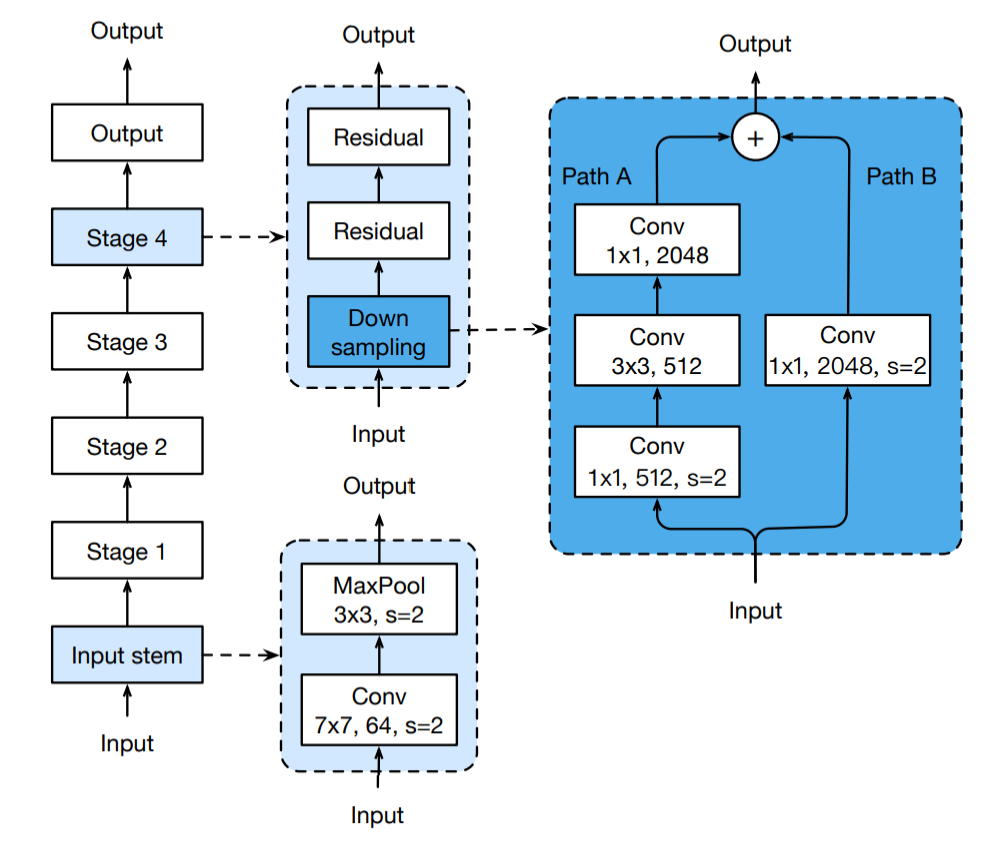
\includegraphics[width=\textwidth]{img/03-resnet_50.png}
        \caption{ResNet-50}
        \label{fig:skip1}
    \end{subfigure}
    \hspace{1cm}
    \begin{subfigure}[b]{0.3\textwidth}
        \centering
        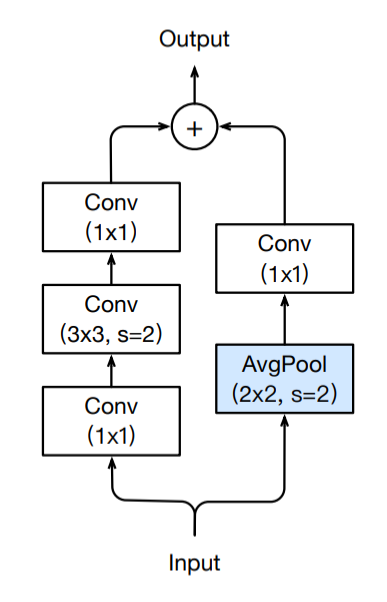
\includegraphics[width=\textwidth]{img/03-resnet_d.png}
        \caption{ResNet-D}
        \label{fig:skip2}
    \end{subfigure}
    \caption{So sánh sự thay đổi của ResNet-D lên block downsampling của ResNet-50}
    \label{fig:resnet_compare}
\end{figure}

\item \textbf{Antialiased Rect-2 Blur Pooling \hyperref[anti-aliased]{(Zhang, 2019)}:} Kỹ thuật này tích hợp các bộ lọc làm mờ (blur filters) vào các lớp downsampling.
\begin{itemize}
\item \textit{Vấn đề răng cưa (Aliasing):} Khi một hình ảnh hoặc bản đồ đặc trưng được downsampling, nếu không được xử lý cẩn thận, hiện tượng aliasing (hiện tượng méo mó tín hiệu do lấy mẫu dưới mức) có thể xảy ra. Hiện tượng aliasing có thể khiến mạng neural học các đặc trưng sai lệch hoặc kém bền vững. Mô hình có thể trở nên nhạy cảm với những thay đổi nhỏ trong vị trí của đối tượng, vì những thay đổi đó có thể tạo ra các "mẫu aliasing" khác nhau, làm cho mạng khó khái quát hóa.
    \begin{figure}[H]
    \centering
        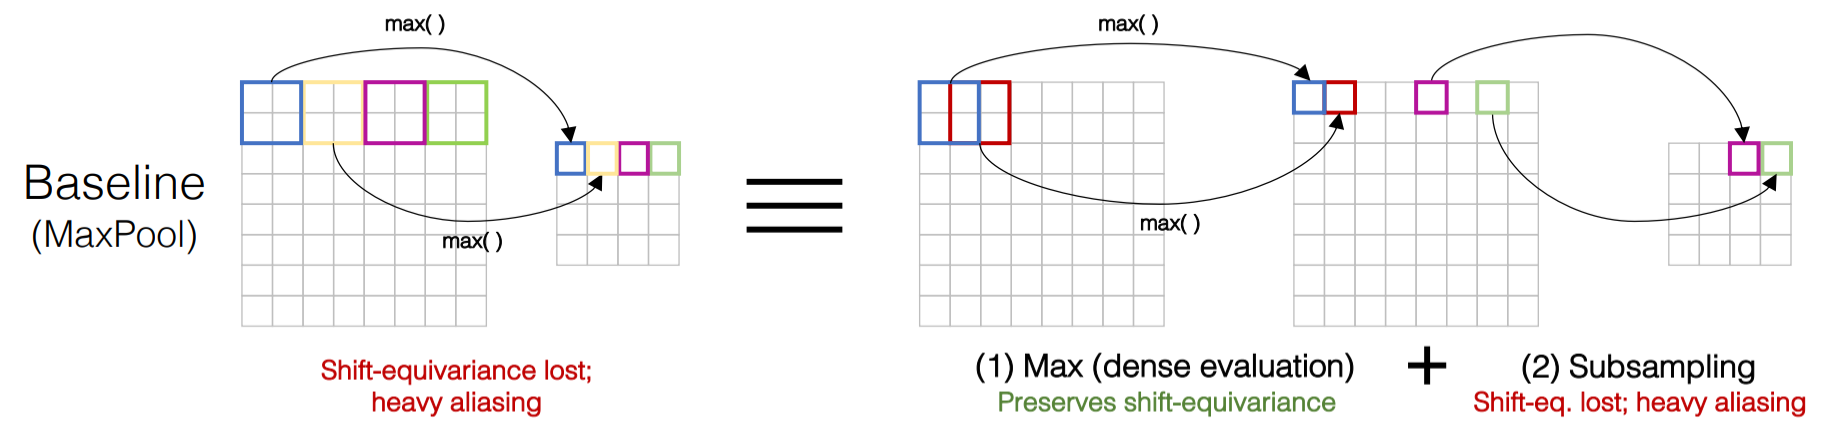
\includegraphics[width=1.0\textwidth]{img/03-maxpool.png}
        \captionsetup{width=0.6\textwidth}
        \caption{Minh họa Max Pooling truyền thống, cho thấy sự mất mát của shift-equivariance và hiện tượng aliasing.}
        \label{fig:maxpool}
    \end{figure}
\item \textit{Giải pháp Blur Pooling:} Bằng cách áp dụng một bộ lọc làm mờ nhỏ trước khi downsampling, Blur Pooling giúp làm mịn các tín hiệu tần số cao có thể gây ra aliasing, làm cho mạng tích chập giữ được tính shift-equivariance (ít nhạy cảm hơn với các dịch chuyển nhỏ). Giữ lại nhiều thông tin hữu ích hơn và làm cho biểu diễn học được mạnh mẽ hơn đối với các biến thể nhỏ trong dữ liệu đầu vào.
    \begin{figure}[H]
    \centering
        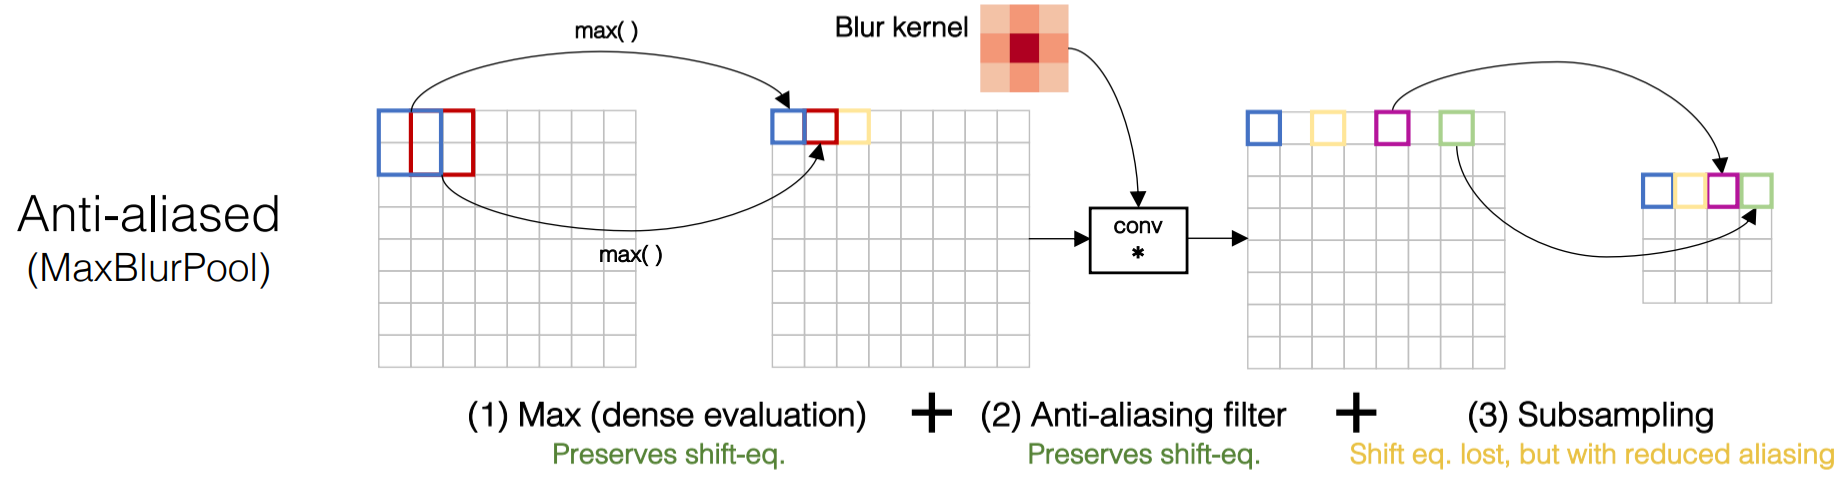
\includegraphics[width=1.0\textwidth]{img/03-blur_pooling.png}
        \captionsetup{width=0.6\textwidth}
        \caption{MaxBlurPool (Anti-aliased), giảm răng cưa bằng cách áp dụng bộ lọc làm mờ trước khi subsampling.}
        \label{fig:blur_pooling}
    \end{figure}
\end{itemize}

Như minh họa, việc mất tính shift-equivariance là không thể tránh khỏi do tính chất của subsampling nhưng bằng cách áp dụng bộ lọc làm mờ trước khi subsampling, hiện tượng aliasing đã được giảm đi đáng kể.
\item \textbf{Thay thế Global Average Pooling bằng Attention Pooling:}

\textit{Global Average Pooling (GAP):} Thường được sử dụng ở cuối mạng CNN để tổng hợp các đặc trưng không gian thành một vector duy nhất bằng cách tính trung bình. Mặc dù đơn giản và hiệu quả trong việc giảm chiều dữ liệu, nó coi mọi thông tin trong feature map đều có mức độ quan trọng như nhau. Điều này có thể khiến mô hình bỏ qua các thông tin quan trọng hoặc tập trung vào các vùng không liên quan trong hình ảnh khi tổng hợp biểu diễn cuối cùng.
    \begin{figure}[H]
    \centering
        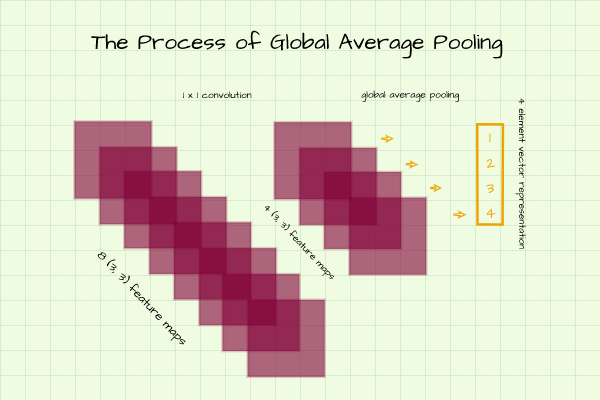
\includegraphics[width=0.7\textwidth]{img/03-global_avg.png}
        \caption{Mỗi feature map sẽ được lấy trung bình để output ra một số duy nhất.}
        \label{fig:global_avg}
    \end{figure}
\textit{Attention Pooling của CLIP:} CLIP thay thế GAP bằng một cơ chế pooling dựa trên attention. Điều này cho phép mô hình học cách "chú ý" có chọn lọc đến các vùng quan trọng nhất của hình ảnh. Đây là một lớp multi-head QKV attention (Query, Key, Value) kiểu "Transformer":
\begin{itemize}
    \item \textbf{Query (Truy vấn):} Trong trường hợp này, vector truy vấn (query) được điều kiện hóa bởi một đặc trưng được tổng hợp bằng Global Average Pooling (GAP) từ feature map đầu vào. Nghĩa là, một bản tóm tắt ban đầu của hình ảnh (từ GAP) sẽ được dùng để "hỏi" các vùng khác của hình ảnh.
    \item \textbf{Key (Khóa) và Value (Giá trị):} Các vector Key và Value được tạo ra từ mỗi vị trí/điểm ảnh trên bản đồ đặc trưng cuối cùng của mạng CNN (trước lớp pooling).
\end{itemize}
Cơ chế này sẽ tính toán "điểm chú ý" giữa vector Query và từng vector Key từ bản đồ đặc trưng. Các điểm chú ý này sau đó được chuẩn hóa thành trọng số, cho biết mức độ "quan trọng" của từng vùng trong hình ảnh. Cuối cùng, một vector biểu diễn duy nhất cho toàn bộ hình ảnh được tạo ra bằng cách lấy tổng có trọng số của các vector Value, với trọng số là các điểm chú ý đã tính.

\textbf{Lợi ích:} Cơ chế attention cho phép mô hình tập trung vào các vùng quan trọng nhất của hình ảnh khi tạo ra biểu diễn cuối cùng. Thay vì trung bình đơn giản, nó "ưu tiên" các thông tin có giá trị cao. Điều này đặc biệt có lợi cho các nhiệm vụ đa phương thức của CLIP. Khi một hình ảnh chứa nhiều đối tượng hoặc bối cảnh phức tạp.

\item \textbf{Chiến lược mở rộng mô hình (Model Scaling):}
\begin{itemize}
\item \textit{Kinh nghiệm từ EfficientNet \hyperref[efficientnet]{(Tan \& Le, 2019)}:} Thay vì chỉ mở rộng một chiều (chiều rộng, chiều sâu hoặc độ phân giải đầu vào), CLIP áp dụng một cách tiếp cận tương tự EfficientNet: phân bổ thêm năng lực tính toán để mở rộng \textbf{đồng thời cả chiều rộng, chiều sâu và độ phân giải đầu vào} của mô hình. Cách tiếp cận này được chứng minh là hiệu quả nhất để cải thiện hiệu suất với một lượng tính toán nhất định.
\item \textit{Các phiên bản ResNet của CLIP:} Từ ResNet-50 cơ sở, CLIP huấn luyện các mô hình lớn hơn, được ký hiệu là RN50x4, RN50x16 và RN50x64. Các ký hiệu này cho thấy mô hình lớn hơn tương ứng 4 lần, 16 lần và 64 lần về số lượng channel so với ResNet-50 ban đầu.
\end{itemize}
\end{enumerate}
\paragraph{Dòng kiến trúc Vision Transformer (ViT)}
Vision Transformer \hyperref[vit]{(Dosovitskiy et al., 2020)} là một kiến trúc tương đối mới tại thời điểm CLIP ra đời, chứng minh rằng Transformer (vốn được thiết kế cho NLP) cũng có thể đạt hiệu suất SOTA trong thị giác máy tính, đặc biệt khi được huấn luyện trên dữ liệu lớn. CLIP cũng khám phá và sử dụng ViT làm bộ mã hóa hình ảnh của mình.
\begin{itemize}
\item \textbf{CLIP tuân thủ khá sát với việc triển khai ViT gốc. Có các sửa đổi nhỏ:}
\begin{itemize}
\item \textit{Thêm lớp Layer Normalization:} Một sửa đổi nhỏ là việc thêm một lớp layer normalization bổ sung vào trước các khối Transformer, sau khi kết hợp các patch và position embeddings. Điều này có thể giúp ổn định quá trình huấn luyện và cải thiện hiệu suất.
    \begin{figure}[H]
    \centering
        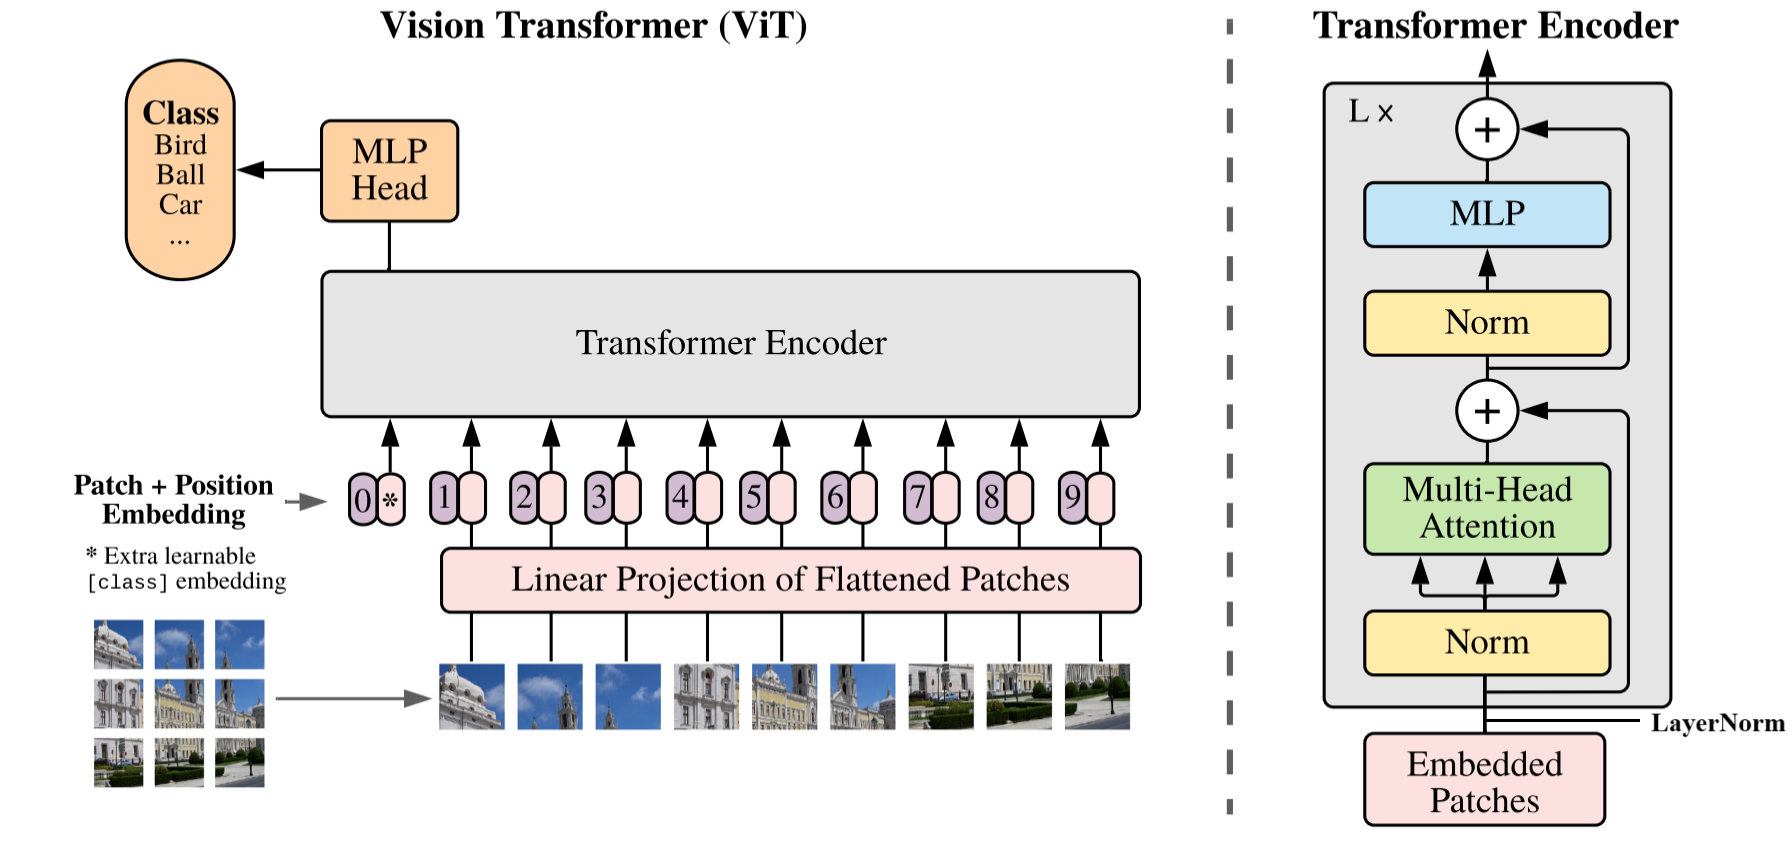
\includegraphics[width=0.9\textwidth]{img/03-vit.png}
        \caption{Thêm LayerNorm sau Embedded Patches trước khi vào Encoder}
        \label{fig:global_avg}
    \end{figure}
\item Áp dụng một lược đồ khởi tạo (initialization scheme) khác một chút.
\end{itemize}
\item \textbf{Hiệu quả tính toán vượt trội:} Các nghiên cứu sau này (cũng như CLIP) đã chỉ ra rằng ViT thường hiệu quả tính toán hơn CNN (như ResNet) khi được huấn luyện trên các bộ dữ liệu rất lớn. Điều này cho phép CLIP đạt được hiệu suất tổng thể cao hơn trong cùng một ngân sách tính toán.
\item \textbf{Các phiên bản ViT của CLIP:} Bao gồm ViT-B/32, ViT-B/16 và ViT-L/14.
\item \textbf{Huấn luyện ở độ phân giải cao hơn (ViT-L/14@336px):} Để tăng cường hiệu suất (tương tự kỹ thuật FixRes), phiên bản ViT-L/14 lớn nhất còn được huấn luyện thêm một epoch ở độ phân giải hình ảnh cao hơn (336x336 pixel) sau khi đã huấn luyện ở độ phân giải tiêu chuẩn (224x224 pixel).
\end{itemize}
\subsubsection{Text Encoder}
\paragraph{}{Bộ mã hóa văn bản của CLIP chịu trách nhiệm biến đổi các đoạn văn bản (chú thích) thành các vector biểu diễn có ngữ nghĩa. CLIP sử dụng kiến trúc Transformer làm nền tảng cho bộ mã hóa văn bản, với một số điều chỉnh cụ thể.}
\paragraph{Kiến trúc Transformer cơ sở} Được xây dựng dựa trên kiến trúc Transformer gốc \hyperref[transformer]{(Vaswani et al., 2017)} và kết hợp các cải tiến đáng kể từ mô hình GPT-2 \hyperref[gpt2]{(Radford et al., 2019)} của OpenAI. Điều này ngụ ý rằng nó là một biến thể của Transformer chỉ có decoder, được thiết kế để xử lý chuỗi văn bản.
\begin{itemize}
\item \textbf{Thông số cấu hình điển hình:}
\begin{itemize}
\item \textit{Số lớp và chiều rộng:} Phiên bản cơ sở thường là mô hình 12 lớp với chiều rộng 512 (512 chiều của các embedding bên trong các khối Transformer).
\item \textit{Attention Heads:} Sử dụng 8 head attention, cho phép mô hình tập trung vào các phần khác nhau của chuỗi đầu vào và học các mối quan hệ đa dạng giữa các từ cùng một lúc, từ đó thu thập được các khía cạnh thông tin phong phú hơn.
\end{itemize}
\item \textbf{Mã hóa văn bản (Text Tokenization):}
\begin{itemize}
\item \textit{Lowercase:} Đầu tiên, tất cả văn bản đầu vào được chuyển đổi sang chữ thường. Bước này giúp giảm độ phức tạp của từ vựng và làm cho mô hình ít nhạy cảm hơn với sự khác biệt về cách viết hoa/thường, coi "Dog" và "dog" là cùng một từ.
\item \textit{Byte Pair Encoding (BPE):} Văn bản đầu vào được mã hóa thành các "tokens" bằng thuật toán BPE \hyperref[bpe]{(Sennrich et al., 2015)}. BPE là một phương pháp nén dữ liệu hiệu quả, kết hợp các ký tự hoặc chuỗi ký tự phổ biến thành các tokens lớn hơn dựa theo từ điển, giúp xử lý các từ hiếm gặp (không nằm trong từ điển) và giảm kích thước từ vựng.
    \begin{figure}[H]
    \centering
        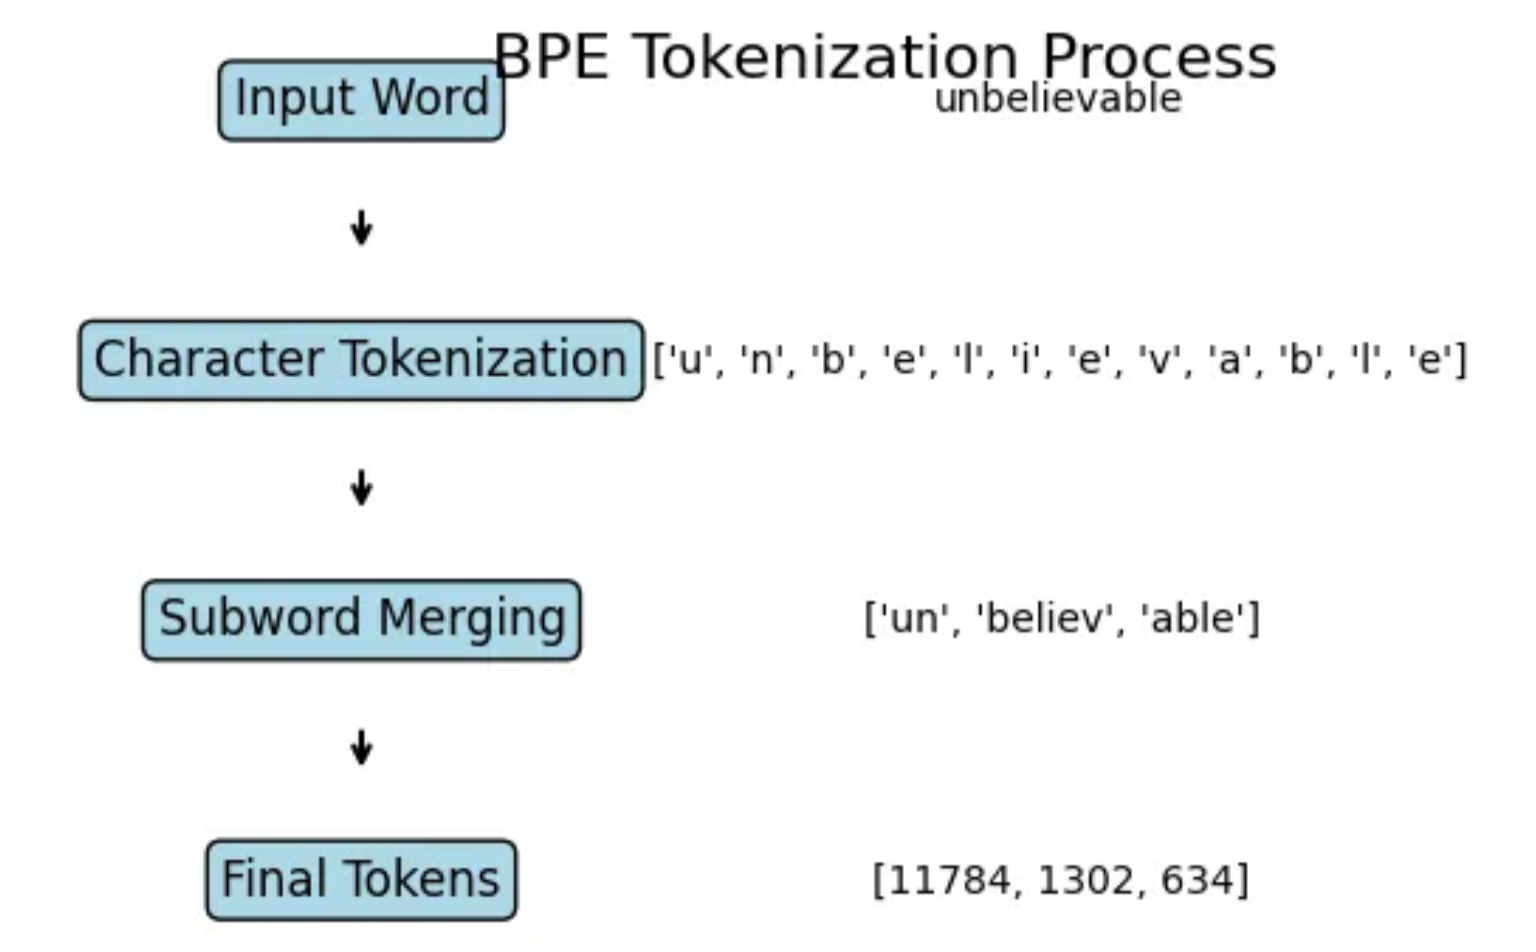
\includegraphics[width=0.7\textwidth]{img/03-bpe.png}
        \captionsetup{width=0.7\textwidth}
        \caption{Các từ phổ biến sẽ được giữ nguyên, trong khi từ ít gặp sẽ được chia nhỏ thành các subwords phổ biến nhất.}
        \label{fig:global_avg}
    \end{figure}
\item \textit{Kích thước từ vựng:} Sử dụng kích thước từ vựng là 49.152.
\item \textit{Token [SOS] và [EOS]:} Mỗi trình tự văn bản được bao bọc bởi các token đặc biệt: [SOS] (Start of Sequence) ở đầu văn bản và [EOS] (End of Sequence) ở cuối văn bản. Việc sử dụng các token này giúp mô hình xác định ranh giới của văn bản đầu vào. 
\item \textit{Giới hạn độ dài trình tự:} Vì hiệu quả tính toán, mỗi trình tự token hóa được giới hạn độ dài tối đa là 76 tokens. Các chuỗi dài hơn sẽ bị cắt bớt, và các chuỗi ngắn hơn sẽ được đệm để đạt đủ độ dài này.
\end{itemize}
\item \textbf{Masked Self-Attention:} Một cơ chế attention trong decoder Transformer đảm bảo rằng khi mô hình xử lý một token ở vị trí t, nó chỉ có thể chú ý đến các token ở vị trí 1 đến t, và không thể "nhìn thấy" các token ở vị trí t+1 trở đi (các token tương lai), đảm bảo rằng việc dự đoán từ tiếp theo trong một chuỗi chỉ dựa trên ngữ cảnh đã biết (các từ trước đó). 

Tuy nhiên, \textbf{CLIP không được huấn luyện để sinh văn bản}. Nhiệm vụ huấn luyện chính của CLIP là học đối lập giữa hình ảnh và văn bản, không phải là dự đoán từ tiếp theo. Sau khi mã hóa, các chuỗi đầu vào sẽ đi qua nhiều lớp Transformer. Mỗi lớp Transformer sẽ xử lý chuỗi bằng các cơ chế Masked Self-Attention. Nhờ cơ chế này, ở mỗi lớp, mỗi token trong chuỗi đều có một vector biểu diễn ngữ cảnh riêng. Vector này không chỉ thể hiện bản thân token đó mà còn mã hóa thông tin về mối quan hệ của nó với các token trước đó trong chuỗi.

\item \textbf{Trích xuất đặc trưng:}

Đây là bước then chốt. Thay vì chỉ quan tâm đến logits của từ tiếp theo, CLIP tận dụng các vector biểu diễn ngữ cảnh này.
\begin{itemize}
\item Biểu diễn đặc trưng của văn bản được lấy từ \textbf{biểu diễn của token [EOS] ở lớp Transformer cuối cùng (lớp cao nhất)}. Token [EOS] thường được coi là một điểm đặc biệt nơi toàn bộ ngữ cảnh của chuỗi đã được tổng hợp. Vector biểu diễn của [EOS] ở lớp cuối cùng thường được coi là một vector biểu diễn toàn diện và ngữ nghĩa của toàn bộ chuỗi văn bản đã được xử lý. Nó đã "nhìn thấy" tất cả các token trước nó và tổng hợp thông tin từ chúng.
\item \textit{Layer Normalization và Linear Projection:} Sau khi trích xuất, vector đặc trưng này được chuẩn hóa lớp và sau đó được chiếu tuyến tính vào một không gian nhúng chung. Đây là không gian mà các vector hình ảnh cũng được chiếu vào, cho phép tính toán độ tương đồng giữa văn bản và hình ảnh.
\end{itemize}
\end{itemize}

\paragraph{Chiến lược mở rộng quy mô:} CLIP nhận thấy rằng hiệu suất tổng thể của nó không quá nhạy cảm với việc tăng số lượng tham số của bộ mã hóa văn bản. Do đó, khi mở rộng quy mô tổng thể của mô hình, họ chủ yếu tập trung vào việc mở rộng \textbf{chiều rộng} của bộ mã hóa văn bản một cách tương ứng với bộ mã hóa hình ảnh (ResNet hoặc ViT), nhưng \textbf{không tăng chiều sâu} (số lớp Transformer) một cách đáng kể. Điều này giúp tối ưu hóa hiệu quả tính toán trong khi vẫn đạt được hiệu suất mạnh mẽ.

\subsection{Tiền huấn luyện với Contrastive Learning}
\label{subsec:contrastive_learning}
\paragraph{}{Đây là yếu tố then chốt tạo nên sự khác biệt về hiệu suất và khả năng mở rộng của CLIP so với các phương pháp trước đó trong việc học biểu diễn thị giác từ ngôn ngữ tự nhiên.}

\subsubsection{Tại sao lại là Contrastive Learning?}

\paragraph{}{Ban đầu, một số phương pháp học biểu diễn hình ảnh từ văn bản (như VirTex) đã cố gắng xây dựng mô hình generative, nghĩa là mô hình sẽ \textbf{dự đoán chính xác chú thích} của một hình ảnh. Tuy nhiên, phương pháp này gặp phải một số thách thức lớn:}
\begin{itemize}
    \item \textbf{Độ phức tạp và tính hiệu quả:} Việc dự đoán từng từ chính xác trong một câu chú thích là một nhiệm vụ rất phức tạp đối với mô hình. Ngôn ngữ có sự đa dạng lớn, nhiều cách diễn đạt, và nhiễu đáng kể trong dữ liệu web (chú thích có thể không luôn hoàn hảo hoặc liên quan trực tiếp đến hình ảnh). Điều này khiến việc huấn luyện mô hình generative trở nên kém hiệu quả về mặt tính toán và khó mở rộng quy mô. Các tác giả cũng đã chuyển sang thử nghiệm một baseline đơn giản hơn: dự đoán một "túi từ" của văn bản (tức là chỉ quan tâm từ nào xuất hiện, không quan tâm thứ tự hay ngữ pháp).
    \begin{figure}[H]
    \centering
        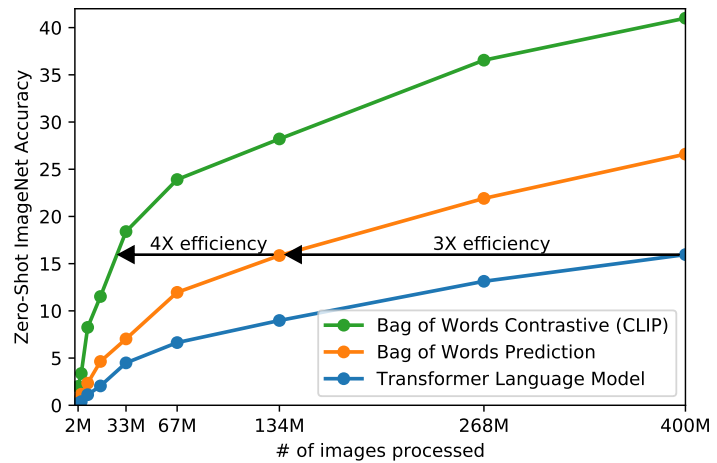
\includegraphics[width=\textwidth]{img/03-zero_shot_comparison.png}
        \captionsetup{width=0.9\textwidth}
        \caption{Trong một so sánh về hiệu năng zero-shot transfer, nhóm nghiên cứu chỉ ra rằng mô hình Transformer dựa trên generative học chậm hơn 3 lần so với baseline dự đoán bag-of-words và thậm chí là chậm hơn 12 lần so với Contrastive learning của CLIP.}
        \label{fig:zero_shot_comparison}
    \end{figure}
    \item \textbf{Tập trung sai mục tiêu:} Mục tiêu cuối cùng là học được biểu diễn hình ảnh hữu ích cho nhiều tác vụ khác nhau, chứ không phải chỉ để tạo ra chú thích hoàn hảo. Đôi khi, việc dự đoán chú thích chính xác có thể khiến mô hình quá tập trung vào các chi tiết ngôn ngữ thay vì mối quan hệ ngữ nghĩa cốt lõi giữa hình ảnh và văn bản.
\end{itemize}
\paragraph{}{Nhận thấy những hạn chế này, nhóm nghiên cứu đã chuyển sang một nhiệm vụ proxy (proxy task) đơn giản hơn nhưng hiệu quả hơn nhiều: \textbf{Contrastive learning}. Ý tưởng này được lấy cảm hứng từ các nghiên cứu gần đây về học biểu diễn đối lập trong các lĩnh vực khác, cho thấy chúng có thể học được biểu diễn tốt hơn so với các mục tiêu dự đoán tương đương (\hyperref[tian]{Tian et al., 2019}; \hyperref[chen]{Chen et al., 2020a}).}

\subsubsection{Cơ chế hoạt động của Contrastive learning trong CLIP}

\begin{enumerate}
    \item \textbf{Xây dựng Batch đầu vào:}
    \begin{itemize}
        \item Trong mỗi bước huấn luyện, một batch gồm $N$ cặp (hình ảnh, văn bản) thực tế được thu thập từ bộ dữ liệu WIT. Ví dụ: (Image$_1$, Text$_1$), (Image$_2$, Text$_2$), ..., (Image$_N$, Text$_N$).
        \item Đây là $N$ cặp "đúng" (positive pairs) được biết là có liên quan đến nhau.
    \end{itemize}

    \item \textbf{Tạo các biểu diễn Embeddings:}
    Các bộ mã hóa ảnh và văn bản sẽ nhiệm vụ trích xuất các đặc trưng riêng biệt từ đầu vào của chúng dưới dạng các vector biểu diễn cấp cao. Mục đích là chuyển đổi các đặc trưng này vào một không gian chung, được gọi là \textbf{Multi-modal Embedding Space}. Bước này được thực hiện thông qua \textbf{linear projection layers}.

    Bước này hoạt động như một "cầu nối" giữa hai phương thức, cho phép chúng được so sánh và tương tác một cách có ý nghĩa.

    \paragraph{Chức năng của các Linear projection layer}

    \begin{itemize}
        \item \textbf{Ánh xạ vào không gian chung:} Mỗi bộ mã hóa (hình ảnh và văn bản) sẽ tạo ra một vector đặc trưng riêng biệt (ví dụ: $I_f$ cho hình ảnh và $T_f$ cho văn bản). Các vector này có thể có số chiều khác nhau và nằm trong các không gian đặc trưng riêng của từng phương thức. Để có thể so sánh trực tiếp chúng, CLIP sử dụng một lớp chiếu tuyến tính riêng biệt cho mỗi phương thức: $W_i$ cho hình ảnh và $W_t$ cho văn bản.
        \begin{itemize}
            \item Cụ thể, đặc trưng hình ảnh $I_f$ sẽ được biến đổi thành $I_e = I_f \cdot W_i$, và đặc trưng văn bản $T_f$ sẽ được biến đổi thành $T_e = T_f \cdot W_t$.
            \item Mục tiêu là $I_e$ và $T_e$ sẽ có cùng số chiều và nằm trong cùng một không gian nhúng đa phương thức.
        \end{itemize}
        \item \textbf{Đầu ra tuyến tính:} Khác với một số mô hình học biểu diễn đối lập khác (ví dụ: SimCLR) thường sử dụng một "projection head" phi tuyến tính (gồm nhiều lớp MLP với hàm kích hoạt phi tuyến tính) để ánh xạ các đặc trưng từ bộ mã hóa vào không gian nhúng, CLIP đã lựa chọn một lớp chiếu \textbf{tuyến tính} đơn giản.
        \begin{itemize}
            \item Điều đáng ngạc nhiên là nhóm nghiên cứu CLIP nhận thấy rằng việc sử dụng lớp chiếu tuyến tính không gây ra sự khác biệt đáng kể về hiệu quả huấn luyện so với lớp chiếu phi tuyến tính.
            \item Điều này gợi ý rằng các biểu diễn đặc trưng mà các bộ mã hóa hình ảnh và văn bản học được (trước khi chiếu) đã có chất lượng rất cao và đủ mạnh mẽ để có thể được ánh xạ tuyến tính vào không gian chung mà vẫn giữ được thông tin quan trọng. Sự đơn giản này cũng góp phần vào hiệu quả và tính dễ mở rộng của mô hình.
        \end{itemize}
    \end{itemize}

    \paragraph{L2 Normalization}

    Sau khi các vector đặc trưng được chiếu tuyến tính vào không gian chung ($I_e$ và $T_e$), một bước quan trọng tiếp theo là \textbf{chuẩn hóa L2} chúng: $I_e = \text{L2\_normalize}(I_e)$ và $T_e = \text{L2\_normalize}(T_e)$.
    \begin{itemize}
        \item \textbf{Đảm bảo độ dài vector là 1:} Chuẩn hóa L2 (chia mỗi vector cho độ dài Euclid của chính nó) đảm bảo rằng tất cả các vector nhúng trong không gian chung đều có độ dài bằng 1.
        \item \textbf{Tầm quan trọng cho Contrastive Loss:} Độ tương đồng cosine là thước đo tiêu chuẩn để đánh giá "độ gần" ngữ nghĩa trong không gian nhúng của CLIP. Việc chuẩn hóa L2 đảm bảo rằng sự tương đồng này chỉ phụ thuộc vào \textbf{góc} giữa các vector (hướng của chúng), chứ không phải vào độ dài hoặc độ lớn. Điều này rất quan trọng cho Contrastive learning, nơi mô hình cố gắng kéo các cặp liên quan lại gần nhau và đẩy các cặp không liên quan ra xa.
    \end{itemize}

    \item \textbf{Tính toán Similarity Matrix:}
    Với $N$ embedding vector hình ảnh và $N$ embedding vector văn bản từ bước trên, chúng ta có thể tạo ra một ma trận độ tương đồng $S$ có kích thước $N \times N$.
    \begin{itemize}
        \item Mỗi phần tử $S_{i,j}$ của ma trận này được tính bằng \textbf{cosine similarity} giữa vector nhúng hình ảnh $I_i$ và vector nhúng văn bản $T_j$ theo công thức tổng quát sau:
        \begin{align*}
            \cos(\theta) = \frac{A \cdot B}{\left\lVert A \right\rVert \left\lVert B \right\rVert}
        \end{align*}
        Do các vector đã được chuẩn hóa L2, $S_{i,j}$ đơn giản là phép nhân vô hướng $I_i \cdot T_j^T$.
        \begin{figure}[H]
            \centering
            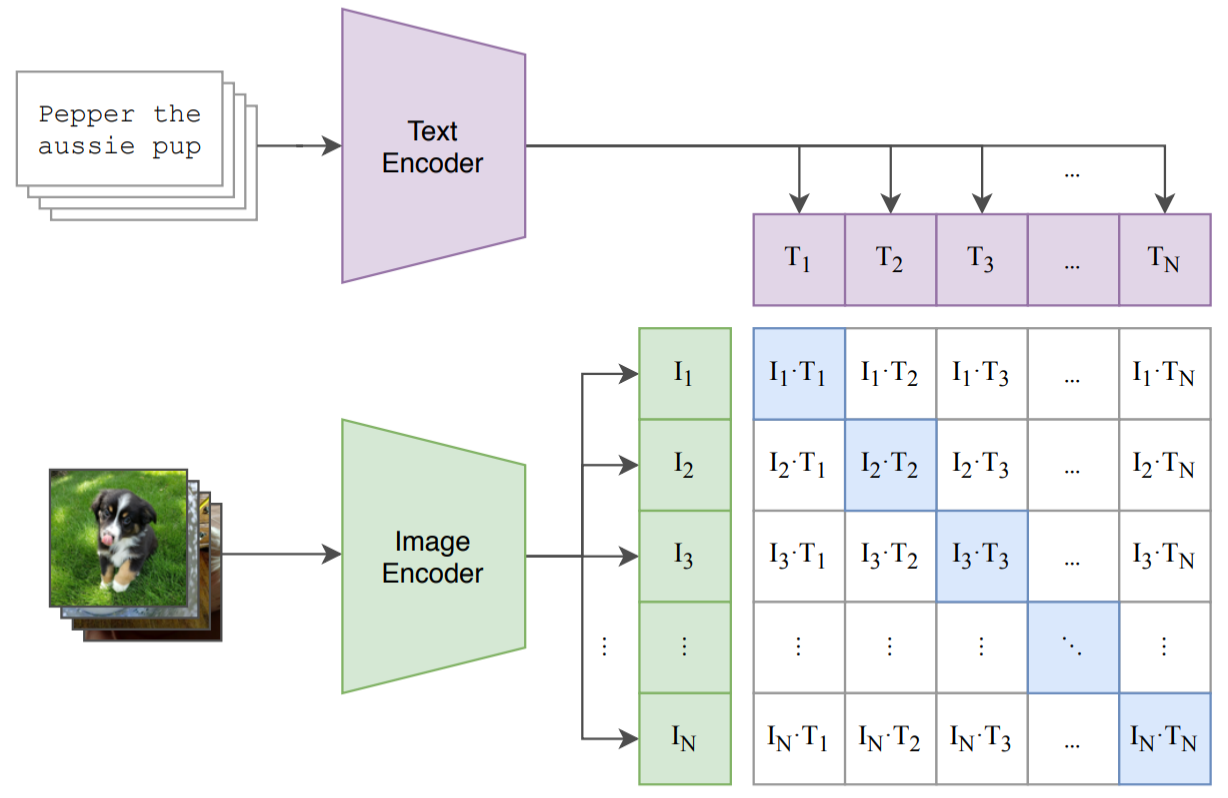
\includegraphics[width=0.9\textwidth]{img/03-similarity_matrix.png}
            \label{fig:zero_shot_comparison}
        \end{figure}
        \item \textit{Ma trận này chứa:}
        \begin{itemize}
            \item Các phần tử trên đường chéo chính $S_{i,i}$ là độ tương đồng giữa các cặp hình ảnh-văn bản \textbf{đúng} (positive pairs).
            \item Các phần tử ngoài đường chéo chính $S_{i,j}$ (với $i \neq j$) là độ tương đồng giữa các cặp hình ảnh-văn bản \textbf{sai} (negative pairs), được tạo ra bằng cách ghép ngẫu nhiên hình ảnh từ một cặp đúng với văn bản từ một cặp đúng khác trong cùng batch.
        \end{itemize}
    \end{itemize}

    \item \textbf{Hàm mất mát và Tối ưu hóa:}
            CLIP sử dụng một phiên bản của mục tiêu học đối lập được gọi là \textbf{N-pair Contrastive Loss} (Sohn, 2016) hoặc \textbf{InfoNCE Loss} (Oord et al., 2018), đã được điều chỉnh cho nhiệm vụ đa phương thức hình ảnh-văn bản (Zhang et al., 2020), được gọi là \textbf{symmetric cross-entropy loss}. Mục tiêu là tối đa hóa độ tương đồng của $N$ cặp đúng trong khi giảm thiểu độ tương đồng của $N^2 - N$ cặp sai.
    \begin{itemize}
        \item \textit{Cụ thể:}
        \begin{itemize}
            \item Mô hình xem xét mỗi hàng của ma trận $S$ như một tập hợp các "logits" (đầu ra thô, chưa qua xử lý) để phân loại hình ảnh $I_i$ với $N$ đoạn văn bản có thể có.
            \item Đồng thời, mô hình xem xét mỗi cột của ma trận $S$ như một tập hợp các "logits" để phân loại văn bản $T_j$ với $N$ hình ảnh có thể có.
            \item Hàm mất mát tổng cộng là trung bình của hàm mất mát cross-entropy từ phía hình ảnh (phân loại văn bản cho ảnh) và từ phía văn bản (phân loại ảnh cho văn bản).
        \end{itemize}
        \item \textbf{Temperature Parameter $t$:}
        \begin{itemize}
            \item Tham số $t$ được sử dụng để điều khiển dải giá trị của các logits trước khi đưa vào hàm softmax (logits được nhân với $\exp(t)$).
            \item Một giá trị $t$ lớn hơn sẽ làm cho phân phối xác suất sau softmax "sắc nét" hơn, tập trung nhiều hơn vào các cặp có độ tương đồng cao nhất.
            \item Điều đặc biệt của CLIP là tham số $t$ này không phải là một siêu tham số cố định mà được \textbf{tối ưu hóa trực tiếp} trong quá trình huấn luyện (được tham số hóa theo log để tránh các giá trị quá lớn gây mất ổn định huấn luyện). Điều này giúp mô hình tự điều chỉnh độ "sắc nét" của sự phân biệt giữa các cặp đúng và sai.
        \end{itemize}
    \end{itemize}
\end{enumerate}

\textbf{Mã giả:}
\begin{figure}[H]
\centering
    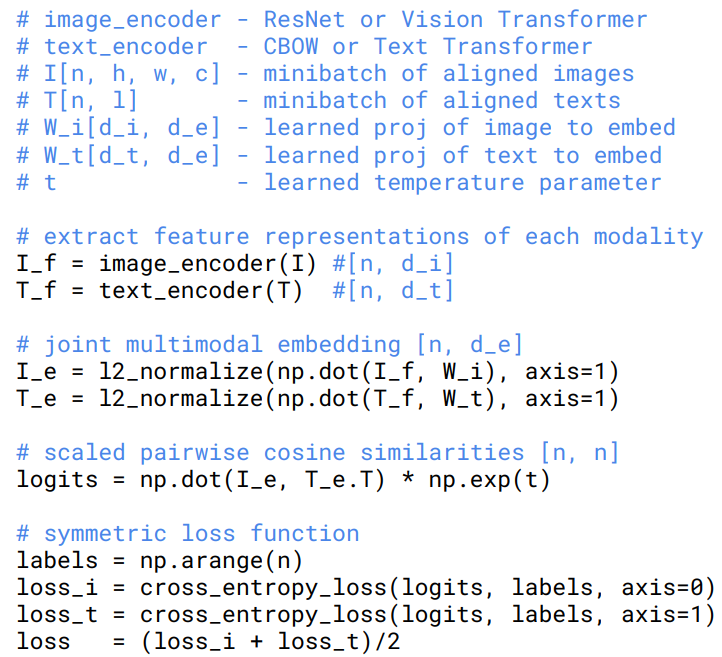
\includegraphics[width=0.7\textwidth]{img/03-pseudocode.png}
    \caption{Mã giả các bước tiến hành CLIP}
    \label{fig:pseudocode}
\end{figure}

\subsection{Đặc điểm của Multi-modal Embedding Space}
\paragraph{}{Đây chính là sản phẩm cuối cùng của quá trình ánh xạ, và là nơi sự "hiểu biết" đa phương thức của CLIP thực sự phát huy tác dụng. Mô hình phải học được sự khác biệt thực sự về khái niệm, chứ không chỉ dựa vào các đặc trưng cấp thấp.}

\begin{itemize}
    \item \textbf{Một không gian thống nhất:} Multi-modal Embedding Space là không gian vector cao chiều, nơi các biểu diễn của hình ảnh và văn bản có thể được so sánh trực tiếp.
    \item \textbf{Phản ánh mối quan hệ ngữ nghĩa:}
    \begin{itemize}
        \item Nếu một hình ảnh và một đoạn văn bản mô tả cùng một khái niệm hoặc có mối quan hệ ngữ nghĩa chặt chẽ (ví dụ: một bức ảnh về một chú mèo và chú thích "a cat napping on the sofa"), các embedding vector tương ứng của chúng ($I_e$ và $T_e$) sẽ nằm \textbf{rất gần nhau} trong không gian này, với độ tương đồng cosine cao.
        \item Ngược lại, nếu một hình ảnh và một đoạn văn bản không có mối quan hệ (ví dụ: một bức ảnh về một chú chó và chú thích "a blue car"), các vector nhúng của chúng sẽ nằm \textbf{xa nhau}, với độ tương đồng cosine thấp.
        
        Điều này minh họa một cách mạnh mẽ rằng việc học để ánh xạ hai phương thức vào một không gian ngữ nghĩa thống nhất là chìa khóa để CLIP có thể tổng quát hóa sang các tác vụ mới chỉ bằng cách sử dụng ngôn ngữ.
    \end{itemize}
    \item \textbf{Khả năng "Open-set" của không gian:} Vì không gian này được học từ dữ liệu ngôn ngữ tự nhiên đa dạng (WIT), nó không bị giới hạn bởi một tập hợp các lớp cố định. Điều này có nghĩa là các khái niệm chưa từng được "nhìn thấy" trong hình ảnh huấn luyện vẫn có thể được hiểu nếu chúng có mô tả bằng ngôn ngữ tương ứng.
\end{itemize}
\newpage
\section{So sánh các biến thể của CLIP}

\paragraph{}{CLIP được huấn luyện với nhiều kiến trúc Image Encoder và kích thước khác nhau, dẫn đến các biến thể với hiệu suất và chi phí tính toán khác nhau.}

\begin{figure}[H]
    \centering
    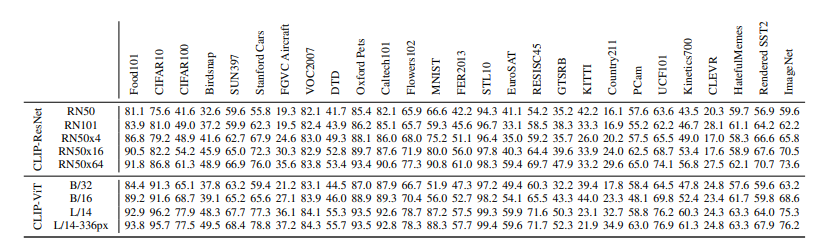
\includegraphics[width=1\linewidth]{img/04-Compare_CLIP.png}
    \caption{Bảng so sánh hiệu suất Zero-shot của các biến thể CLIP trên 17 tập dữ liệu}
\end{figure}

\paragraph{}{Dựa vào bảng so sánh trên, ta có các nhận xét:}
\begin{itemize}
    \item Scaling Laws: Hiệu suất của CLIP tăng lên đáng kể khi tăng kích thước mô hình (cả Image Encoder và Text Encoder) và lượng dữ liệu huấn luyện.
    \item ViT vs. ResNet: Các mô hình Vision Transformer (ViT) thường cho hiệu suất tốt hơn so với các mô hình ResNet có cùng lượng tính toán, đặc biệt là ở quy mô lớn.
    \item Zero-Shot Power: Ngay cả các biến thể nhỏ hơn của CLIP cũng cho thấy khả năng zero-shot ấn tượng trên nhiều bộ dữ liệu và tác vụ khác nhau, vượt xa các phương pháp trước đó.
    \item Tính toán và bộ nhớ: Các mô hình lớn hơn (như ViT-L/14) đòi hỏi tài nguyên tính toán và bộ nhớ GPU đáng kể cho cả huấn luyện và suy luận.
\end{itemize}

\section{Ưu điểm, thách thức}
\paragraph{Ưu điểm nổi bật}{
\begin{itemize}
    \item \textbf{Khả năng Zero-Shot mạnh mẽ:} Đây là đóng góp quan trọng nhất, cho phép áp dụng vào nhiều tác vụ thị giác mà không cần huấn luyện lại hoặc fine-tuning.
    \item \textbf{Học từ dữ liệu web tự nhiên:} Giảm sự phụ thuộc vào các bộ dữ liệu được gán nhãn thủ công tốn kém.
    \item \textbf{Tính linh hoạt cao:} Dễ dàng thích ứng với các tác vụ mới chỉ bằng cách thay đổi mô tả văn bản (prompt engineering).
    \item \textbf{Mô hình nền tảng (Foundation Model):} Có thể được sử dụng làm cơ sở cho nhiều ứng dụng downstream phức tạp hơn (ví dụ: tạo ảnh từ văn bản, VQA).
    \item \textbf{Robustness:} Hiệu suất tốt trên nhiều loại dữ liệu và phân phối khác nhau so với các mô hình chỉ học trên tập dữ liệu cố định.
\end{itemize}
}

\paragraph{Thách thức, hạn chế:}{
\begin{itemize}
    \item \textbf{Khó khăn với tác vụ chi tiết:} CLIP có thể gặp khó khăn với các tác vụ đòi hỏi sự hiểu biết rất chi tiết, ví dụ như đếm số lượng đối tượng nhỏ, nhận diện chữ rất nhỏ (fine-grained OCR), hoặc các mối quan hệ không gian phức tạp.
    \item \textbf{Chi phí tính toán:} Huấn luyện CLIP đòi hỏi tài nguyên tính toán rất lớn. Các mô hình lớn nhất cũng tốn kém khi suy luận.
    \item \textbf{Độ nhạy với Prompt Engineering:} Hiệu suất có thể thay đổi đáng kể tùy thuộc vào cách diễn đạt câu truy vấn văn bản.
    \item \textbf{Dữ liệu "nhiễu" và thiên kiến (Bias):} Vì học từ dữ liệu web, CLIP có thể kế thừa các thiên kiến xã hội tiềm ẩn trong dữ liệu đó.
    \item \textbf{Không phải là "All-in-one":} Mặc dù mạnh mẽ, CLIP không phải lúc nào cũng là lựa chọn tốt nhất cho mọi tác vụ thị giác. Các mô hình chuyên biệt được huấn luyện có giám sát vẫn có thể vượt trội trong các lĩnh vực hẹp cụ thể.
    \item \textbf{Khả năng trừu tượng hóa hạn chế:} Gặp khó khăn khi khái quát hóa với các khái niệm hoàn toàn mới hoặc trừu tượng mà không có sự tương đồng trong dữ liệu huấn luyện
\end{itemize}
}
% Slide 1
\section{Ứng dụng của CLIP}
\begin{frame}{5. Ứng dụng của CLIP}
\begin{itemize}
    \item \textbf{Truy vấn} giữa ảnh và văn bản (Text-to-Image, Image-to-Text Retrieval)
    \item Nâng cao: \textbf{Phân biệt khuôn mặt}, từ đó phát triển tác vụ nhận diện khuôn mặt người.
\end{itemize}
\end{frame}

\begin{frame}{5.1 Ứng dụng của CLIP trong truy vấn giữa ảnh và văn bản}
\begin{itemize}
    \item Text-to-Image, Image-to-Text Retrieval
    \item CLIP hỗ trợ truy vấn đa chiều: từ văn bản tìm ảnh, hoặc từ ảnh tìm văn bản mô tả tương ứng.
    \item Ví dụ: Gõ “người đàn ông đeo kính” → truy xuất ảnh phù hợp trong tập dữ liệu.
    \item Ứng dụng trong tìm kiếm hình ảnh, gợi ý nội dung, kiểm duyệt nội dung tự động,...
\end{itemize}
\end{frame}

\begin{frame}{5.1.1 Giới thiệu bộ dữ liệu COCO 2017}
\begin{itemize}
    \item \textbf{COCO} (Common Objects in Context) là bộ dữ liệu chuẩn cho nhiều bài toán thị giác máy tính: phát hiện đối tượng, phân đoạn ảnh, và truy xuất ảnh từ văn bản.
    
    \item \textbf{Số lượng:}
    \begin{itemize}
        \item \textbf{Train2017:} 118.000 ảnh có gán nhãn.
        \item \textbf{Val2017:} 5.000 ảnh dùng để đánh giá mô hình.
        \item \textbf{Test2017:} 41.000 ảnh (không có nhãn công khai).
    \end{itemize}

    \item \textbf{Chú thích:} Mỗi ảnh đi kèm trung bình 5 câu mô tả tự nhiên (caption) — phù hợp cho huấn luyện/truy vấn ảnh-văn bản.

    \item \textbf{Định dạng:} Ảnh '.jpg' và nhãn định dạng '.json' (COCO-style annotations).

    \item \textbf{Ứng dụng:} Được dùng rộng rãi trong huấn luyện và đánh giá mô hình như CLIP, BLIP, Flamingo, ViLT,...
\end{itemize}
\end{frame}

\begin{frame}{5.1.2 Thực hiện bài toán truy vấn với CLIP (ViT-B/32)}
\textbf{Ghi chú:} Do bài toán yêu cầu huấn luyện trên tập dữ liệu lớn và đòi hỏi tài nguyên GPU đáng kể, mô hình CLIP đã được huấn luyện sẵn bởi OpenAI là một lựa chọn phù hợp và hiệu quả.

\vspace{1em}
\textbf{Các bước thực hiện:}
\begin{itemize}
    \item \textbf{Bước 1:} Nạp mô hình CLIP ViT-B/32 được huấn luyện sẵn từ thư viện OpenAI.
    \item \textbf{Bước 2:} Tiền xử lý ảnh và văn bản đầu vào (chuẩn hóa kích thước, token hóa văn bản).
    \item \textbf{Bước 3:} Trích xuất vector đặc trưng (embedding) cho cả ảnh và văn bản thông qua mô hình CLIP.
    \item \textbf{Bước 4:} Tính độ tương đồng cosine giữa các vector đặc trưng để đo mức độ phù hợp.
    \item \textbf{Bước 5:} Truy xuất kết quả phù hợp nhất: tìm ảnh gần nhất với truy vấn văn bản, hoặc ngược lại.
\end{itemize}
\end{frame}

\begin{frame}{5.1.3 Kết quả và Nhận xét trên tập COCO}
\textbf{Kết quả đánh giá trên tập COCO validation:}
\begin{itemize}
    \item \textbf{Recall@1:} 49.92\%
    \item \textbf{Recall@5:} 74.94\%
    \item \textbf{Recall@10:} 83.24\%

\end{itemize}

\vspace{0.5em}
\textbf{Nhận xét:}
\begin{itemize}
    \item CLIP đạt kết quả tốt với Recall@10 trên 83\%, cho thấy khả năng định vị đúng ảnh nằm trong top đầu là rất cao.
    \item Recall@1 còn hạn chế ($\sim$ 50\%) – mô hình có thể nhầm khi truy vấn có ngữ nghĩa gần nhau.
    \item Phù hợp với ứng dụng cần độ bao phủ cao (top-5/top-10), cần cải tiến thêm nếu yêu cầu chính xác tuyệt đối.
\end{itemize}
\end{frame}

\begin{frame}{5.1.4 Ví dụ minh hoạ kết quả truy vấn}
\begin{columns}
    % Cột trái: hình ảnh
    \begin{column}{0.5\textwidth}
        \centering
        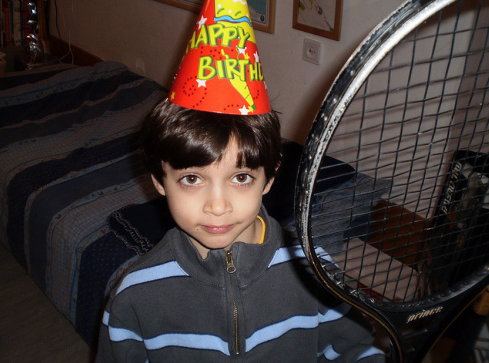
\includegraphics[width=0.95\linewidth]{img/05-imagecaption.png} % Thay bằng đường dẫn ảnh thật
        \vspace{0.5em}
        \textit{Ảnh minh hoạ truy vấn}
    \end{column}

    % Cột phải: truy vấn và caption
    \begin{column}{0.5\textwidth}
        \textbf{Truy vấn văn bản:} 
         \begin{itemize}
        \item “A boy in birthday hat holding a tennis racket” , 
        \item "A boy swinging a tennis racket at a ball on a court."
        \end{itemize}

        \vspace{1em}

        \textbf{Caption gốc:}
        \begin{itemize}
            \item “A boy in birthday hat holding a tennis racket"
            \item "A young boy in a birthday hat holds a tennis racquet”
        \end{itemize}
    \end{column}
\end{columns}
\end{frame}

\begin{frame}{5.2 Ứng dụng CLIP để phân biệt khuôn mặt người}
\begin{itemize}
    \item CLIP học mối liên hệ giữa ảnh và văn bản từ hàng trăm triệu cặp dữ liệu.
    \item Dù không thiết kế riêng cho nhận diện khuôn mặt, CLIP có khả năng biểu diễn ảnh mạnh mẽ.
\end{itemize}
\textbf{Mục tiêu}
\begin{itemize}
    \item Mã hóa ảnh khuôn mặt thành vector đặc trưng (embedding).
    \item Dự đoán và phân biệt khuôn mặt bằng cách so sánh độ tương đồng giữa các embedding.
\end{itemize}
\end{frame}

% Slide 2
\begin{frame}{5.2.1 Dữ liệu}
\textbf{Dữ liệu:} Kaggle Face Recognition Dataset
\begin{itemize}
    \item Dựa trên LFW, ảnh 250x250 JPG.
    \item Mỗi thư mục tương ứng với một người nổi tiếng (2–50 ảnh).
\end{itemize}
\textbf{Xử lý dữ liệu:}
\begin{enumerate}
    \item Tăng cường dữ liệu (augmentation).
    \item Chia thành Train/Test.
    \item Tạo Dataloader với cặp ảnh.
\end{enumerate}
\begin{figure}
    \centering
    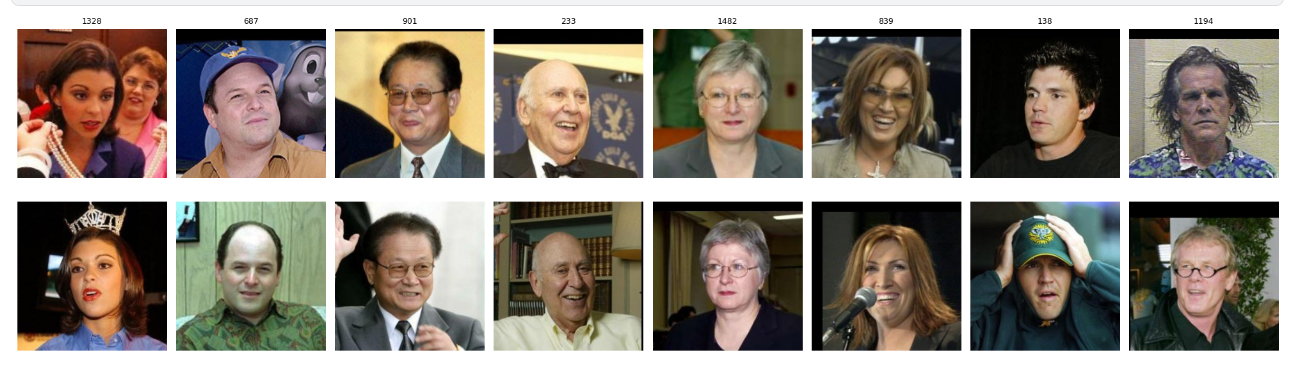
\includegraphics[width=0.75\linewidth]{img/05-Face.png}
    \caption{Ví dụ khuôn mặt trong tập dữ liệu.}
\end{figure}
\end{frame}

% Slide 3
\begin{frame}{5.2.2 Sử dụng lớp VisionTransformer từ ViT-B/32 (CLIP)}
\begin{columns}
    \begin{column}{0.62\textwidth}
        \begin{itemize}
        \item \textbf{Patch Embedding:} Ảnh chia thành các patch kích thước $32 \times 32$ và chuyển thành vector.
    \item \textbf{LayerNorm:} Chuẩn hóa đầu vào cho Transformer.
    \item \textbf{Transformer Encoder:} Gồm 12 khối ResidualAttentionBlock:
    \begin{itemize}
        \item Mỗi block có multi-head attention với đầu vào/ra 768 chiều.
        \item Chuẩn hóa (\texttt{ln\_1}, \texttt{ln\_2}).
        \item MLP: Linear(768 $\rightarrow$ 3072) $\rightarrow$ QuickGELU $\rightarrow$ Linear(3072 $\rightarrow$ 768).
    \end{itemize}
    \item \textbf{Output LayerNorm:} Chuẩn hóa để lấy embedding có đầu ra 768.
        \end{itemize}
    \end{column}
    \begin{column}{0.25\textwidth}
        \centering
        \begin{figure}
            \centering            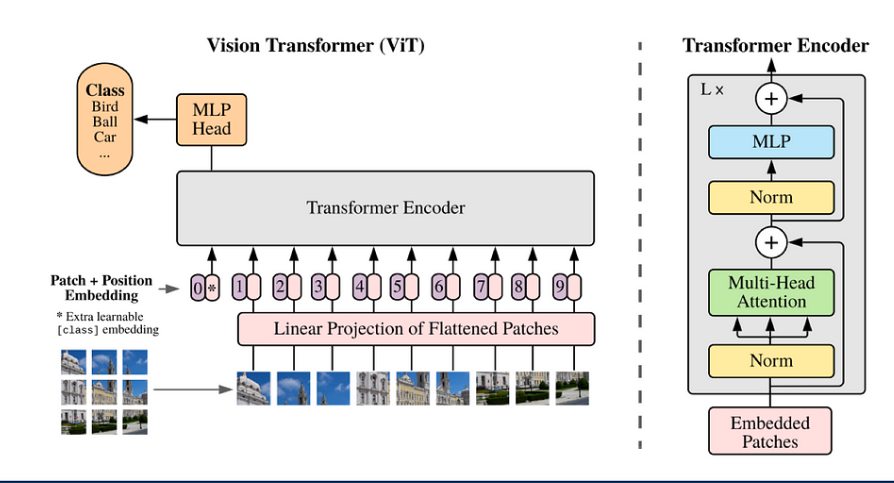
\includegraphics[width=\linewidth]{img/05-visontransformer.png} 
            \tiny Kiến trúc mạng Vision Transformer
        \end{figure}
    \end{column}
\end{columns}
\end{frame}


\begin{frame}{5.2.3 Huấn luyện và Đánh giá mô hình ViT}
\begin{columns}
    % Cột trái: mô tả
    \begin{column}{0.5\textwidth}
        \small % �� Chữ nhỏ hơn bình thường
        \begin{itemize}
            \item \textbf{Loss:} Contrastive Loss
            \item \textbf{Optimizer:} Adam (learning rate = $1 \times 10^{-3}$)
            \item \textbf{Epoch:} 3
            \item \textbf{Các cặp ảnh:} cùng người, khác người
            \item \textbf{Nhận xét:}
            \begin{itemize}
                \item Sau 3 epoch, loss giảm, mô hình chưa hội tụ. Embedding vector giữa các lớp chưa đủ tách biệt.
                \item Khả năng phân biệt ảnh khác người còn yếu, dẫn đến precision thấp trên tập test. Mô hình dễ nhầm lẫn các cặp không cùng người. F1-score ở mức trung bình cho thấy cần cải thiện thêm.
            \end{itemize}
        \end{itemize}
    \end{column}

    % Cột phải: biểu đồ + bảng
    \begin{column}{0.5\textwidth}
        \begin{figure}
            \centering
            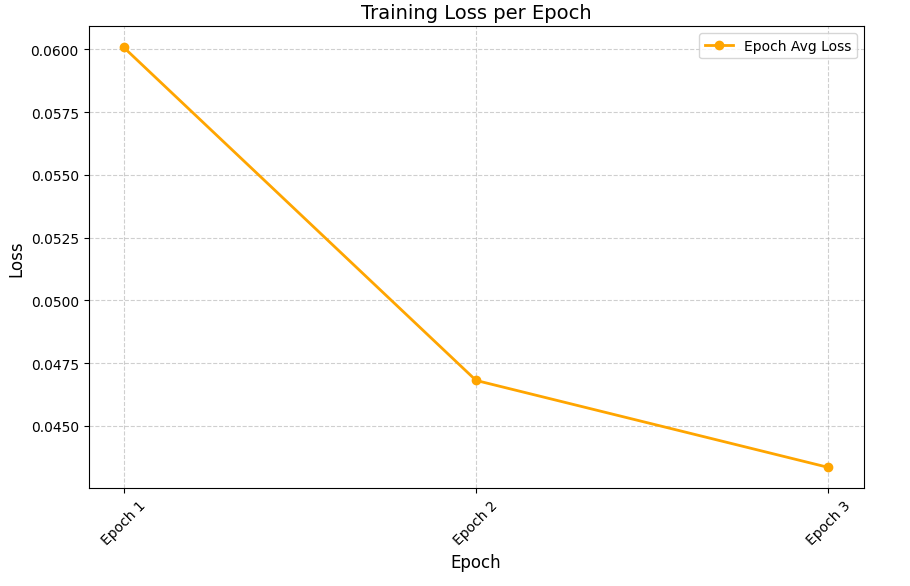
\includegraphics[width=0.8\linewidth]{img/05-loss.png}
        \end{figure}
        \begin{center}
        \scriptsize
        \begin{tabular}{|l|c|c|}
            \hline
            \textbf{Chỉ số} & \textbf{Train} & \textbf{Test} \\
            \hline
            Accuracy  & 72.92\% & 71.65\% \\
            Precision & 83.56\% & 66.76\% \\
            Recall    & 57.06\% & 86.24\% \\
            F1-score  & 67.81\% & 75.26\% \\
            \hline
        \end{tabular}
        \end{center}
    \end{column}
\end{columns}
\end{frame}

\begin{frame}{5.2.4 Kết quả ảnh test}
\vspace{-0.5em}

\begin{minipage}[t]{0.48\textwidth}
    \centering
    \begin{figure}
    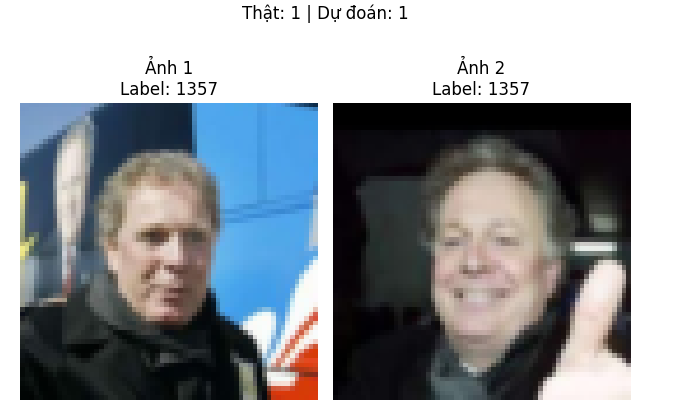
\includegraphics[width=0.95\linewidth]{img/05-1.png}
    {Khoảng cách: 0.1810\\Thật: 1, Dự đoán: 1}
    \end{figure}
\end{minipage}
\hfill
\begin{minipage}[t]{0.48\textwidth}
    \centering
    \begin{figure}
        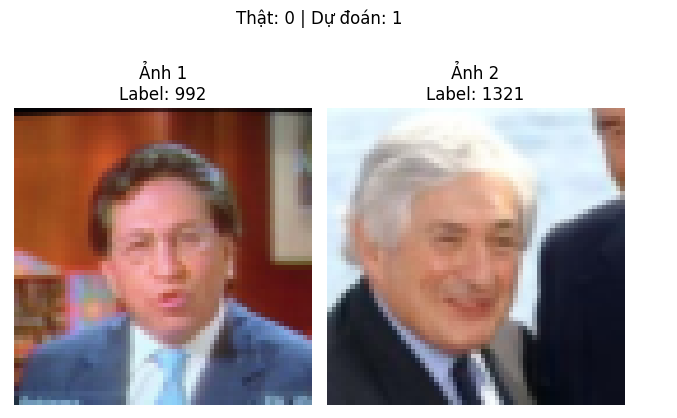
\includegraphics[width=0.95\linewidth]{img/05-2.png}
        {Khoảng cách: 0.1999\\Thật: 0, Dự đoán: 1}
    \end{figure}
        
\end{minipage}

\begin{itemize}
    \item  Tính \textbf{Khoảng cách} giữa hai vector đặc trưng ảnh.
    \item Nếu khoảng cách $<$ \textbf{0.2} thì hai ảnh được dự đoán là \textbf{cùng nhãn}.
\end{itemize}
\end{frame}


\begin{frame}{5.2.5 So sánh với mô hình CNN khác trong tác vụ phân biệt khuôn mặt người}
\footnotesize
Mặc dù không được thiết kế chuyên biệt cho tác vụ phân biệt khuôn mặt người, mô hình vẫn đạt hiệu quả cao nhờ chiến lược: \textbf{trích xuất embedding cho toàn bộ ảnh, tính khoảng cách, và gán nhãn theo ảnh gần nhất trong tập dữ liệu đã biết.}
\begin{table}[H]
\centering
\begin{tabular}{|c|c|c|c|c|}
\hline
\textbf{Mô hình} & Accuracy & Precision & Recall & F1 \\
\hline
CLIP (ViT-B/32) & \textbf{0.73} & \textbf{0.6982} & \textbf{0.7311} & \textbf{0.7022} \\
ResNet18        & 0.2151           & 0.1743           & 0.2151          & 0.1672          \\
ResNet50        & 0.2169           & 0.1493         & 0.2169          & 0.1483          \\
EfficientNet-B0 & 0.2218           & 0.1658           & 0.2218          & 0.1621          \\
MobileNetV2     & 0.2602           & 0.1916          & 0.2602         & 0.1923         \\
\hline
\end{tabular}
\end{table}
\begin{itemize}
    \item CLIP pretrained mang lại hiệu suất cao, không cần huấn luyện lại.
    \item Ưu tiên sử dụng CLIP nếu tài nguyên tính toán cho phép.
\end{itemize}
\end{frame}


\newpage
\section{Các mô hình tương tự CLIP}

\subsection{ALIGN} 

\paragraph{}{Trong phương pháp \textbf{ALIGN} được giới thiệu trong bài báo \textbf{Scaling Up Visual and Vision-Language Representation Learning With Noisy Text Supervision} \cite{jia2021scalingvisualvisionlanguagerepresentation}, các biểu diễn (representations) hình ảnh và ngôn ngữ được huấn luyện đồng thời từ dữ liệu nhiễu (noisy) là các cặp ảnh và văn bản thay thế (alt-text). Các bộ mã hóa hình ảnh (image encoder) và văn bản (text encoder) được học thông qua hàm mất mát tương phản (contrastive loss), được định dạng dưới dạng softmax chuẩn hóa. Hàm mất mát này có tác dụng đẩy các embedding của cặp ảnh-văn bản khớp nhau lại gần nhau hơn, đồng thời đẩy chúng ra xa các embedding của những cặp ảnh-văn bản không khớp.\\

% Mô hình học cách căn chỉnh (align) các biểu diễn hình ảnh và ngôn ngữ của các cặp ảnh-văn bản bằng cách sử dụng hàm mất mát tương phản. Các biểu diễn này có thể được sử dụng để chuyển giao cho các tác vụ chỉ liên quan đến thị giác (vision-only) hoặc các tác vụ ngôn ngữ-thị giác (vision-language). Không cần bất kỳ tinh chỉnh (fine-tuning) nào, ALIGN có thể thực hiện phân loại hình ảnh zero-shot và tìm kiếm chéo phương thức (cross-modal search), bao gồm tìm kiếm từ ảnh sang văn bản, từ văn bản sang ảnh, và thậm chí tìm kiếm với các truy vấn kết hợp cả ảnh và văn bản.
}

\begin{figure}[H]
    \centering
    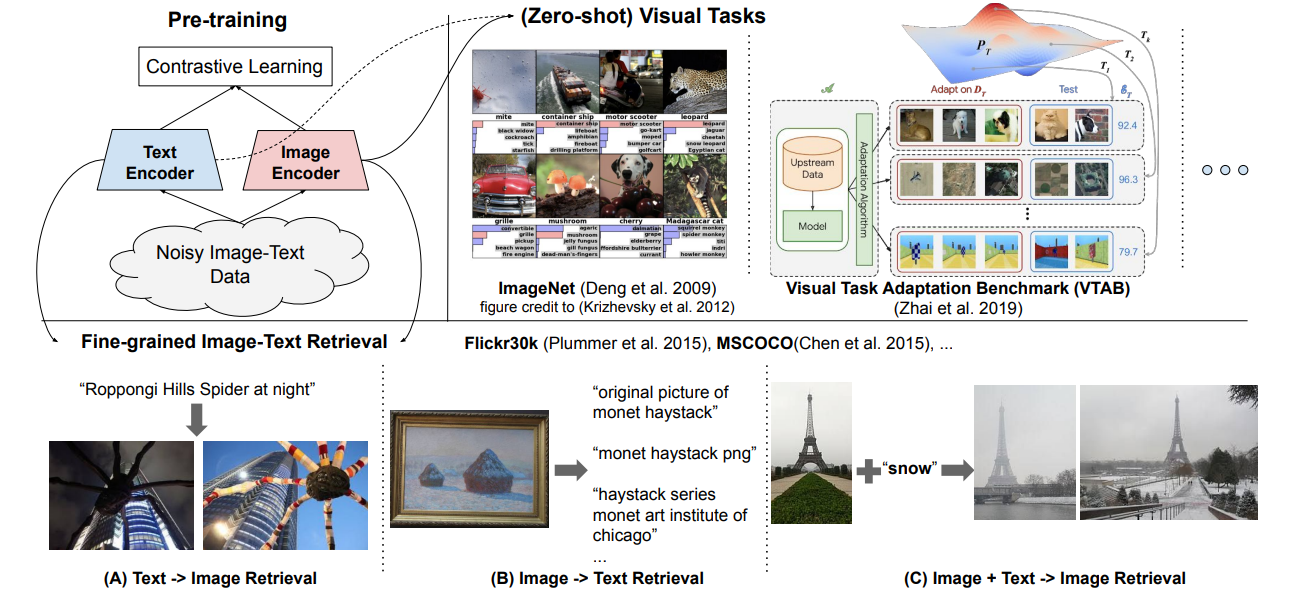
\includegraphics[width=1\linewidth]{img/06-ALIGN.png}
    \caption{Tóm tắt phương pháp ALIGN.}
\end{figure}

\paragraph{}{\textbf{Mục tiêu chính:} Mục tiêu của ALIGN là học các biểu diễn (representations) mạnh mẽ cho cả thị giác (vision) và ngôn ngữ-thị giác (vision-language) bằng cách mở rộng quy mô dữ liệu huấn luyện lên mức cực lớn, nhưng với một phương pháp thu thập dữ liệu đơn giản, ít tốn kém. Giả thuyết cốt lõi của họ là \textbf{quy mô của dữ liệu có thể bù đắp cho sự nhiễu} của nó.}

\paragraph{}{\textbf{Kĩ thuật chính:}}

\begin{itemize}
    \item \textbf{Dữ liệu (Data)}: Đây là điểm đột phá và khác biệt nhất của ALIGN. 
    \begin{itemize}
        \item \textbf{Nguồn}: Họ sử dụng một tập dữ liệu khổng lồ gồm hơn 1.8 tỷ cặp ảnh và alt-text (văn bản thay thế cho ảnh) được thu thập từ web.

        \item \textbf{Đặc điểm}: Dữ liệu này rất "nhiễu" (noisy). Các alt-text thường không phải là mô tả hoàn hảo, có thể chứa thông tin không liên quan, tên file, hoặc chỉ là một vài từ khóa.

        \item \textbf{Quy trình lọc}: Thay vì áp dụng các bước lọc và xử lý phức tạp, tốn kém như các bộ dữ liệu được giám sát kỹ lưỡng (ví dụ: Conceptual Captions), ALIGN chỉ áp dụng các bộ lọc rất đơn giản dựa trên tần suất (frequency-based filtering). Ví dụ: loại bỏ các ảnh/văn bản khiêu dâm, ảnh có kích thước quá nhỏ, hoặc các alt-text quá phổ biến (như "ảnh"), quá ngắn hoặc quá dài.
    \end{itemize}

    \item \textbf{Kiến trúc mô hình (Model architecture)}:
    \begin{itemize}
        \item ALIGN sử dụng một kiến trúc \textbf{bộ mã hóa kép (dual-encoder)}.

        \item \textbf{Image Encoder}: Một mạng CNN, cụ thể là \textbf{EfficientNet}.

        \item \textbf{Text Encoder}: Một mạng Transformer, cụ thể là \textbf{BERT}.

        \item Kiến trúc này lấy một ảnh và một đoạn văn bản, mã hóa chúng một cách độc lập để tạo ra hai vector embedding.
    \end{itemize}

    \item \textbf{Hàm mục tiêu (Loss function)}:
    \begin{itemize}
        \item Cả Image encoder và Text encoder được huấn luyện bằng một \textbf{hàm mất mát tương phản (contrastive loss)}, cụ thể là normalized softmax loss (còn gọi là InfoNCE).
        \item \textbf{Cách hoạt động}: Trong một batch dữ liệu, với mỗi cặp (ảnh, văn bản) đúng, mô hình sẽ cố gắng kéo vector embedding của chúng lại gần nhau trong không gian biểu diễn chung. Đồng thời, nó sẽ đẩy embedding của cặp đó ra xa khỏi tất cả các embedding của các ảnh và văn bản khác trong batch (được coi là các cặp "âm" - negative pairs). Quá trình này giúp "căn chỉnh" (align) không gian biểu diễn của ảnh và văn bản.
    \end{itemize}

\end{itemize}

\subsection{BLIP}
\paragraph{}{BLIP được giới thiệu trong bài báo \textbf{BLIP: Bootstrapping Language-Image Pre-training for Unified Vision-Language Understanding and Generation} \cite{li2022blipbootstrappinglanguageimagepretraining}. Các mô hình tiền huấn luyện thị giác-ngôn ngữ (Vision-Language Pre-training, viết tắt là VLP) đã nâng cao hiệu suất cho nhiều tác vụ thị giác-ngôn ngữ. Tuy nhiên, hầu hết VLP chỉ vượt trội ở một trong hai tác vụ: \textbf{hiểu} (understanding) hoặc \textbf{sinh} (generation). BLIP là mô hình có thể làm tốt ở cả hai nhiệm vụ này. BLIP còn có phiên bải cải tiến là BLIP-2 \cite{li2023blip2bootstrappinglanguageimagepretraining}.}

\paragraph{}{\textbf{Mục tiêu chính:}}

\begin{itemize}
    \item \textbf{Về mô hình:} Các mô hình hiện có thường chỉ xuất sắc ở một trong hai loại tác vụ: hoặc là các tác vụ \textbf{hiểu} (understanding) như truy xuất ảnh, phân loại (dựa trên kiến trúc encoder), hoặc là các tác vụ \textbf{sinh} (generation) như tạo chú thích ảnh (dựa trên kiến trúc encoder-decoder). BLIP muốn tạo ra một mô hình \textbf{thống nhất (unified)} có thể làm tốt cả hai.
    \item \textbf{Về dữ liệu:} Các mô hình như ALIGN và CLIP đạt được thành công bằng cách tăng quy mô dữ liệu với các cặp (ảnh, alt-text) nhiễu từ web. BLIP cho rằng đây chưa phải là cách tối ưu và đề xuất một phương pháp \textbf{chủ động cải thiện chất lượng dữ liệu} thay vì chỉ chấp nhận sự nhiễu loạn của nó.
\end{itemize}

\begin{figure}[H]
    \centering
    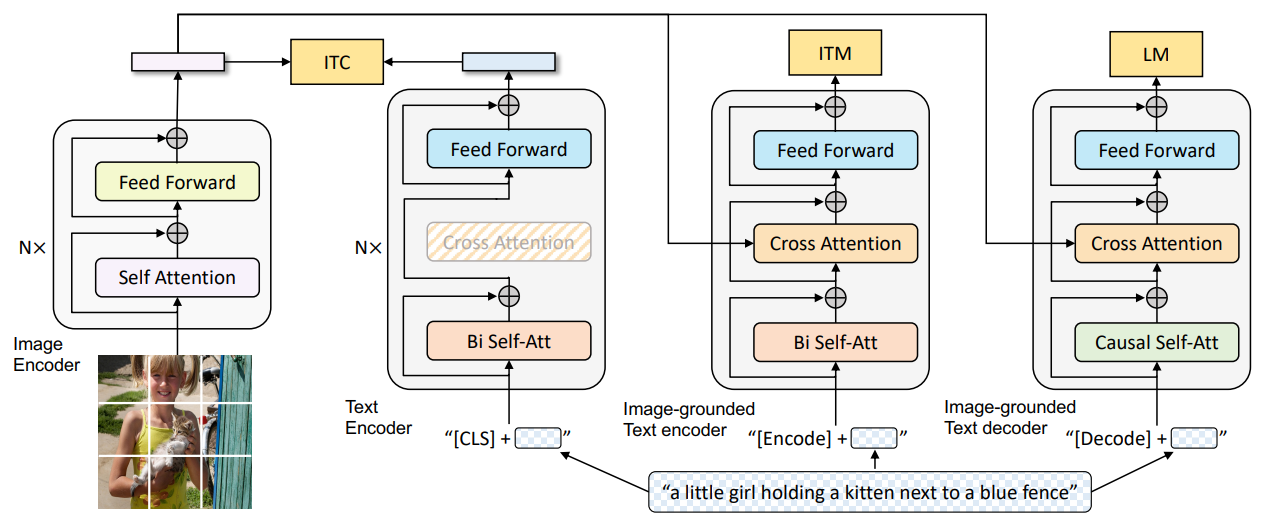
\includegraphics[width=1\linewidth]{img/06-BLIP.png}
    \caption{Tổng quan mô hình BLIP}
\end{figure}

\paragraph{}{\textbf{Kỹ thuật chính:} BLIP giới thiệu hai đóng góp chính - về dữ liệu và về kiến trúc mô hình.}

\begin{itemize}
    \item \textbf{CapFilt (Captioning and Filtering) - Tự cải thiện dữ liệu:} Đây là ý tưởng đột phá nhất của BLIP, một quy trình "bootstrapping" để làm sạch và làm giàu dữ liệu.
    \begin{enumerate}
        \item \textbf{Huấn luyện mô hình ban đầu:} Đầu tiên, họ huấn luyện một mô hình BLIP cơ bản trên 14 triệu cặp ảnh-văn bản nhiễu từ web.
        \item \textbf{Tạo hai mô-đun chuyên dụng:} Từ mô hình đã huấn luyện, họ tinh chỉnh (fine-tune) để tạo ra hai mô-đun: 
        \begin{itemize}
            \item \textbf{Captioner} (Bộ tạo chú thích): Một bộ giải mã (decoder) có khả năng tạo ra các chú thích mới (synthetic captions) cho các ảnh trên web.
            \item \textbf{Filter} (Bộ lọc): Một bộ mã hóa (encoder) học cách xác định xem một cặp (ảnh, văn bản) có khớp nhau hay không.
        \end{itemize}
        \item \textbf{Cải thiện dữ liệu:}
        \begin{itemize}
            \item \textbf{Sinh chú thích mới:} Dùng Captioner để tạo một chú thích mới cho mỗi ảnh từ web.
            \item \textbf{Lọc nhiễu:} Dùng Filter để loại bỏ những cặp (ảnh, văn bản) không khớp. Quá trình lọc này được áp dụng cho cả chú thích gốc từ web và chú thích mới được tạo ra.
        \end{itemize}
        \item \textbf{Huấn luyện mô hình cuối cùng}: Họ kết hợp tập dữ liệu đã được làm sạch và làm giàu này với các bộ dữ liệu chất lượng cao có sẵn (như COCO) để huấn luyện một mô hình BLIP mới từ đầu.
    \end{enumerate}

    Kết quả là họ có một tập dữ liệu huấn luyện lớn, vừa sạch hơn, vừa đa dạng hơn về mặt ngữ nghĩa.

    \item \textbf{MED (Multimodal Mixture of Encoder-Decoder) - Kiến trúc thống nhất:} Để phục vụ cả tác vụ hiểu và sinh, BLIP đề xuất một kiến trúc đa năng có thể hoạt động ở ba chế độ:
    \begin{enumerate}
        \item \textbf{Encoder đơn phương thức (Unimodal Encoder)}: Hoạt động như ALIGN/CLIP. Mã hóa ảnh và văn bản một cách riêng biệt, sau đó dùng contrastive loss (ITC) để căn chỉnh chúng. Dùng cho tác vụ truy xuất.
        \item \textbf{Bộ mã hóa văn bản dựa trên ảnh (Image-grounded Text Encoder)}: Thêm các lớp chú ý chéo (cross-attention) để kết hợp thông tin hình ảnh vào biểu diễn văn bản. Dùng hàm loss image-text matching (ITM) để học sự tương hợp ở mức độ chi tiết hơn (xác định cặp ảnh-văn bản là "positive" hay "negative"). Dùng cho tác vụ hiểu sâu hơn.
        \item \textbf{Bộ giải mã văn bản dựa trên ảnh (Image-grounded Text Decoder)}: Sử dụng các lớp tự chú ý nhân quả (causal self-attention) để sinh văn bản dựa trên ảnh đầu vào. Dùng hàm loss Language Modeling (LM). Dùng cho tác vụ sinh văn bản như tạo chú thích, trả lời câu hỏi.
        
    \end{enumerate}

    Kiến trúc này rất thông minh ở chỗ nó chia sẻ phần lớn các tham số giữa ba chế độ, giúp việc huấn luyện hiệu quả.
\end{itemize}

\subsection{So sánh CLIP, ALIGN và BLIP}

\begin{table}[H]
{%
\begin{tabular}{|l|p{4.5cm}|p{4.5cm}|p{4.5cm}|}
\hline
\textbf{Tính năng} & \textbf{ALIGN (Google)} & \textbf{CLIP (OpenAI)} & \textbf{BLIP (Salesforce)} \\ \hline
Triết lý & Quy mô dữ liệu bù đắp sự nhiễu & Đặt nền móng cho các tác vụ zero-shot. & Linh hoạt, hiểu sâu ảnh-văn bản. \\ \hline
Kiến trúc & EfficientNet - BERT. & Resnet/ViT-Transformer & MED \\ \hline
Dữ liệu & 1.8 tỷ cặp ảnh-văn bản thô từ web. & 400 triệu cặp ảnh-văn bản (WIT). & Tự tạo và lọc dữ liệu (CapFilt). \\ \hline
Thế mạnh & - NLP đa dạng. \newline - Truy vấn rộng& - Phân loại Zero-shot. \newline - Retrieval image. & - Image captioning. \newline - VQA. \\ \hline
Ứng dụng & Hệ thống tìm kiếm hình ảnh bằng ngôn ngữ tự nhiên, phức tạp. & Tác vụ phân loại nhanh mà không cần fine-tuning. & Ứng dụng đòi hỏi sự hiểu biết chi tiết hình ảnh-văn bản. \\ \hline
\end{tabular}%
}
\end{table}



\section{Kết luận}
\begin{frame}{7. Kết luận}
    \begin{block}{CLIP (Contrastive Language-Image Pre-Training)}
    \begin{itemize}
        \item \textbf{CLIP}: Hiểu nội dung hình ảnh và văn bản theo cách liên kết chúng lại với nhau.
        \item \textbf{Mô hình}: Dual-Encoder (ViT/ResNet, Transformer), huấn luyện bằng Contrastive Learning, dựa trên dữ liệu WIT.
        \item \textbf{Ứng dụng}: Phân loại (Zero-shot); truy vấn ảnh (bằng văn bản); làm nền tảng cho caption ranking, VQA.
        \item \textbf{Hạn chế:} Không hỗ trợ sinh văn bản.
    \end{itemize}
  \end{block}
\end{frame}

\newpage
\bibliographystyle{unsrt}
\bibliography{ref/ref}

\appendix
\section{Phụ lục}
\begin{itemize}
\item Template này \textbf{không phải} là template chính thức của Khoa Công nghệ thông tin - Trường Đại học Khoa học Tự nhiên.
\item Các hình ảnh, bảng biểu, thuật toán trong template chỉ mang tính chất ví dụ.
\item Nhóm tác giả phân phối \textbf{miễn phí} template này \href{https://github.com/khongsomeo/hcmus-unofficial-report-template}{trên GitHub} và \href{https://www.overleaf.com/latex/templates/hcmus-report-template/zyrhmsxynwqs}{trên Overleaf} với \href{https://github.com/khongsomeo/hcmus-unofficial-report-template/blob/main/LICENSE}{Giấy phép GNU General Public License v3.0}. Nhóm tác giả không chịu trách nhiệm với các bản phân phối không nằm trong hai kênh phân phối chính thức nêu trên.
\end{itemize}


\end{document}